\documentclass[12pt]{article}%
\usepackage{amsfonts}
\usepackage{fancyhdr}
\usepackage[hidelinks]{hyperref}
\usepackage[a4paper, top=2.5cm, bottom=2.5cm, left=2.2cm, right=2.2cm]%
{geometry}
\usepackage{times}
\usepackage{caption}
\usepackage{subcaption}
\usepackage{amsmath}
\usepackage{nccmath}
\usepackage{listings,newtxtt}
\usepackage{changepage}
\usepackage{amssymb}
\usepackage[titletoc]{appendix}
\usepackage{biblatex}
\usepackage{hyperref}
\usepackage{graphicx}%
\usepackage{float}
\usepackage[nottoc,numbib]{tocbibind}
\addbibresource{references.bib}
\settocbibname{References}
\setcounter{MaxMatrixCols}{30}
\newtheorem{theorem}{Theorem}
\newtheorem{corollary}[theorem]{Corollary}
\newtheorem{definition}[theorem]{Definition}
\newtheorem{lemma}[theorem]{Lemma}
\newtheorem{proposition}[theorem]{Proposition}
\newenvironment{proof}[1][Proof]{\textbf{#1.} }{\ \rule{0.5em}{0.5em}}

\begin{document}
\title{NBA Team and Player Rankings using Networks\\
\vspace{3 mm}
\large ELE/COS 381 Project Report}
\author{Daniel Chae \& Drey Tengan}
\date{\today}
\maketitle

\tableofcontents
\newpage
\section{Introduction and Problem Statement}
\subsection{Introduction and Background}
\null\quad\quad In class, we learned about the PageRank algorithm \cite{PageRank} that allows search engines like Google to efficiently navigate a complex network of webpages based on importance scores. Stemming from our common interest in sports, we were drawn to the idea of applying the PageRank algorithm to sports, specifically to the National Basketball Association (NBA).\\
\null\quad\quad Currently, there exist many metrics that analyze the performance of teams, one primary metric being their win-loss records. Furthermore, there are numerous analysts attempting to predict the outcome of future NBA games and the NBA Playoffs. However, very few of these efforts involve complex networks - most rely on quantiative and qualitative features of teams (e.g. team X has player Y, who has excelled in offense and defense). In fact, in the NBA Power Rankings website, there is a statement: ``NBA.com's Power Rankings, released every Monday during the season, are just one man's opinion. If you have an issue with the rankings, or have a question or comment for John Schuhmann, send him an e-mail or contact him via Twitter'' \cite{nbapowerrating}. This statement indicates that there is some fundamental human-level bias that cannot be waived away. Given the potential of the vast amount of performance data available, more reliable, systematic predictions can be made using the PageRank algorithm or variations on the algorithm.\\
\null\quad\quad Vincent Xia and Kavirath Jain, students of a previous semester of ELE 381, used the PageRank algorithm to predict outcomes of games and rankings of teams in the National Football League (NFL) and the National Basketball Association (NBA) \cite{XJ}. They compared performance of teams and created a predictive ranking of teams using two methods: baseline and weighted (discussed further in Section \ref{sec:relatedwork}). While their procedure yielded about 0.6-0.65 accuracy rate for NFL games, it was less predictive for NBA games. In his 2012 book \textit{The Success Equation}, Michael J. Mauboussin \cite{nbapredictable} claims that of the five major U.S. sports, basketball is the easiest to predict and the most dependent on skill rather than luck, with American football being the ``luckiest'' sport besides hockey. This indicates that there is room to improve analysis and prediction for teams in the NBA, considering that the $0.6-0.65$ accuracy range is just above $0.5$ accuracy, which is just as good as just randomly guessing outcomes.
\subsection{Related Work}
\label{sec:relatedwork}
\null\quad\quad One of the earliest works applying the PageRank algorithm to sports team rankings was by Anjela Govan, Carl Meyer, and Russell Albright in 2008 \cite{Govan}. They implemented a new method for initializing the adjacency matrix for the PageRank algorithm. Suppose there are two teams, team $i$ and team $j$. For every single game that team $i$ beat team $j$, sum up the point differentials. Graphically this sum would be the edge weight going from node $j$ to node $i$. Meaning, node $i$ is receiving from node $j$ to increase its importance score in the algorithm. In the adjacency matrix, the sum would be placed in row $j$, column $i$: $A[j,i]=w_{ij}$, where $w_{ij}$ is the total point differential for all the games that team $i$ beat team $j$. \\
\null\quad\quad As discussed in the previous section, Xia and Jain were students of a previous semester of ELE 381 and they primarily used two methods: baseline and weighted. The baseline method creates an indicator adjacency matrix for the PageRank algorithm. Suppose there are two teams, team $i$ and team $j$. If at any point in the season, team $i$ had beaten team $j$, then for adjacency matrix $A$, $A[j,i]=1$. Graphically, if $i$ and $j$ are nodes, then there is a directed edge from $j$ to $i$ with weight $1$. Otherwise, there is no edge (indicated by $A[j,i]=0$). The weighted method in Xia and Jain is an adaptation of the GeM method in Govan et al. \cite{Govan}. In addition to these two primary methods, Xia and Jain incorporated recency bias into their analysis. If a team continually wins, then there is momentum built in favor of the winning team. In order to account for momentum, they applied $\lambda=0.95$ \cite{XJ} to scale down the most recent victories. Using this recency scheme in conjunction with their weighted method, they were able to improve their accuracy from $62\%$ to $66\%$. 

\subsection{Problem Statement}
\label{sec:1.2}
\null\quad\quad We used network structures, algorithms, and data to better predict the outcome of NBA games. Xia and Jain's weighted method was used as a control and we offer two new alternative ranking methods: Average Point Differential (APD) and Deviant Baseline (DB). We also propose a novel post-processing method: Pick on Someone Your own Size (PSYS). All of these methods are further detailed in Section \ref{sec:2} of this report. After models were trained, we used sequential accuracy testing (discussed in Section \ref{teamimp_networks}) to study the accuracies of the models.\\
\null\quad\quad Another main component of this study is player analysis. Xia and Jain focused on the performance and ranking of teams as a whole. We expand the analysis to consider specific players and their performance against players from other teams. This is an effort that has not been algorithmically attempted. We break this down into two major components: team-pair and All-Star. For team-pair analysis, we select two teams and create networks amongst the players of the two teams using their their box plus minus (+/-), a rating that indicates a player's overall contribution to the game against that team. The goal is to determine the set of players on both teams that would maximize their own team's performance in the game. For All-Star analysis, we create a network on +/- for every single player in the NBA. The network seeks to rank all players in the NBA to determine the best player in the league, best players for each team, and the best players on the Eastern and Western Conferences. These components are further discussed in Section \ref{sec:2}.

\section{Dataset and Networks}
\label{sec:2}
\subsection{Dataset and Scraping Data}
\null\quad\quad Data was obtained from \href{https://www.basketball-reference.com/}{Basketball-Reference.com}, a site that condenses official NBA stats (verified with official stats available from ESPN.com) in a way that is more conducive for the scraping algorithm. We focused on the 30 NBA teams and all 540 players in the 2018-19 season. As mentioned in the Problem Statement, (Section \ref{sec:1.2}) the study analyzes two major sets of networks. One set of networks looks to study team performances against other teams. The goal was to generate a ranking of the teams. This is further explored in Section \ref{sec:2.2}. The second set of networks looks to study individual players against players from other teams, further discussed in Section \ref{sec:2.3}. \\
\null\quad\quad The data was scraped using the BeautifulSoup Python package, stored in pandas DataFrames, manipulated on NumPy, and saved as csv files. The exact solution implementation is further discussed in Section \ref{teamimp_scraping}, Section \ref{playerimp_scraping}, and in the code Appendix.
\subsection{Team Ranking Networks}
\label{sec:2.2}
\null\quad\quad First, team networks were created to compare the performance of teams as a whole and determine the rankings of teams using different methods. The exact implementation is discussed in Section \ref{teamimp_networks}. Each of methods were used to create a network matrix $A$, which is then row-normalized to yield \textbf{H}, which is then used to generate importance scores, $\pi_i$, for each of the methods numbered $i=\{1,2,3,4\}$, using the PageRank algorithm. For the sake of illustrating the four methods, suppose there are only three teams, Golden State Warriors (GSW), Houston Rockets (HOU), and Minnesota Timberwolves (MIN), with match outcomes specified in Table 1.
\begin{center}
\captionof{table}{An example set of matches for the three teams}
\begin{tabular}{|c|c|c|c|}
\hline
\textbf{Team 1} & \textbf{Team 2} & \textbf{Score} & \textbf{Winner}\\
\hline
Warriors & Rockets & 86-107 & Rockets\\
Rockets & Timberwolves & 91-103 & Timberwolves\\
Warriors & Rockets & 104-106 & Warriors\\
Warriors & Timberwolves & 116-99 & Warriors\\
Rockets & Timberwolves & 111-121 & Timberwolves\\
\hline
\end{tabular}
\end{center}
\subsubsection{Weighted Method}
  \null\quad\quad The weighted method is the same weighted method used by Xia and Jain \cite{XJ}. It was employed for the analysis as a control. Suppose there is a square matrix $A$ and let $A_{}[i,j]$ denote the entry of team $i$ against team $j$, where $i$ denotes rows and $j$ denotes columns. Then each of the entries are
  \[
  A_{1}[i,j]=
  \begin{cases}
  \sum_{N_{i\rightarrow j}}d_{ij} &\text{ $i$ lost to $j$}\\
  0 &\text{ otherwise}
  \end{cases}
  \]
  Each of the entries $(i,j)$ is a sum of the point differentials, $d_{ij}$, of the $N$ games where team $i$ lost to team $j$. Graphically, if team $i$ and team $j$ were nodes, then there would be a directed edge from $j$ to $i$ with weight $d_{ij}$. Using the example setup indicated in Table 1, we have the network shown in Figure 1 and the network matrix $A_1$, which is row-normalized to get $\textbf{H}_1$.
  \begin{figure}[H]
	\centering
	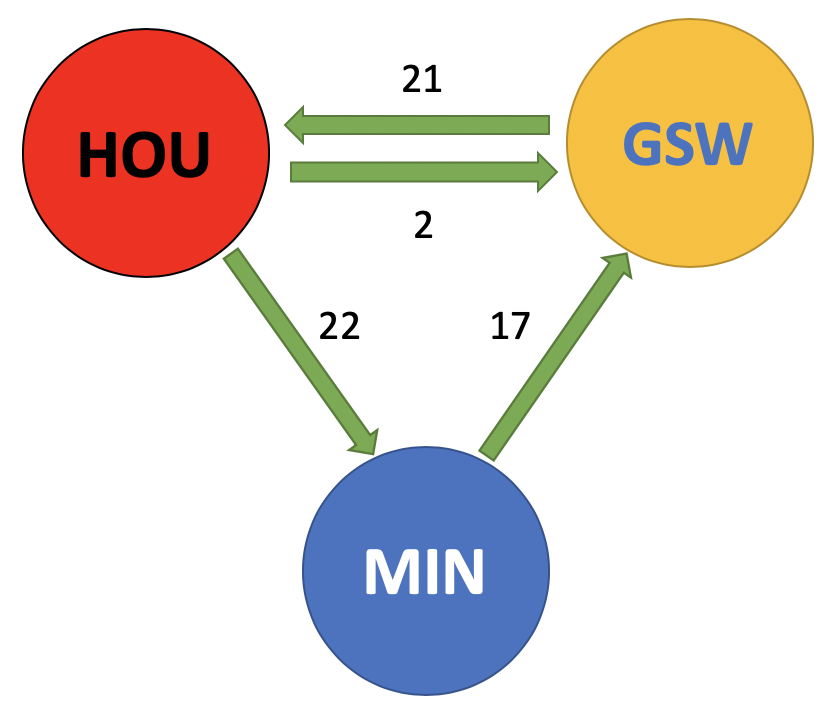
\includegraphics[width=2in]{./images/weighted.png}
	\caption[Network using the Weighted Method]{Network using the Weighted Method}
\end{figure}
\begin{align*}
A_1 =\begin{bmatrix}0 & 21 & 0\\2 & 0 & 22\\17 & 0 & 0\end{bmatrix}, \textbf H_1=\begin{bmatrix}0 & 1 & 0\\0.0833 & 0 & 0.9167\\1 & 0 & 0\end{bmatrix}
\end{align*}

\subsubsection{Average Point Differential (APD)}
  \null\quad\quad The APD method is a newly devised extension of Xia and Jain's weighted algorithm that takes the entries in the weighted method and divides it by the number of games associated with the entries. This is shown by 
  \[
  A_{2}[i,j]=
  \begin{cases}
  \frac{\sum_{N_{i\rightarrow j}}w_{ij,N}}N &\text{ $i$ lost to $j$}\\
  0 &\text{ otherwise}
  \end{cases}
  \]
  Using the example setup, we get the network shown in Figure 2. The motivation behind using this method is to generate directed edges that would scale down deviant blowout games. Meaning, if team $A$ beat team $B$ 5 times with point differential $d_{BA}=\{3,5,2,4,21\}$, the last game with differential $21$ will be scaled down so that the performance of $B$ against $A$ is better indicated with the average of $7$. Graphically, there would be a directed edge going from node $B$ to node $A$ with weight $7$. We take the average instead of the median because we want to leverage the sensitivity of the average to outliers - we still want to indicate that there have been blowout games while still indicating ``average'' performance. 
  \begin{figure}[H]
	\centering
	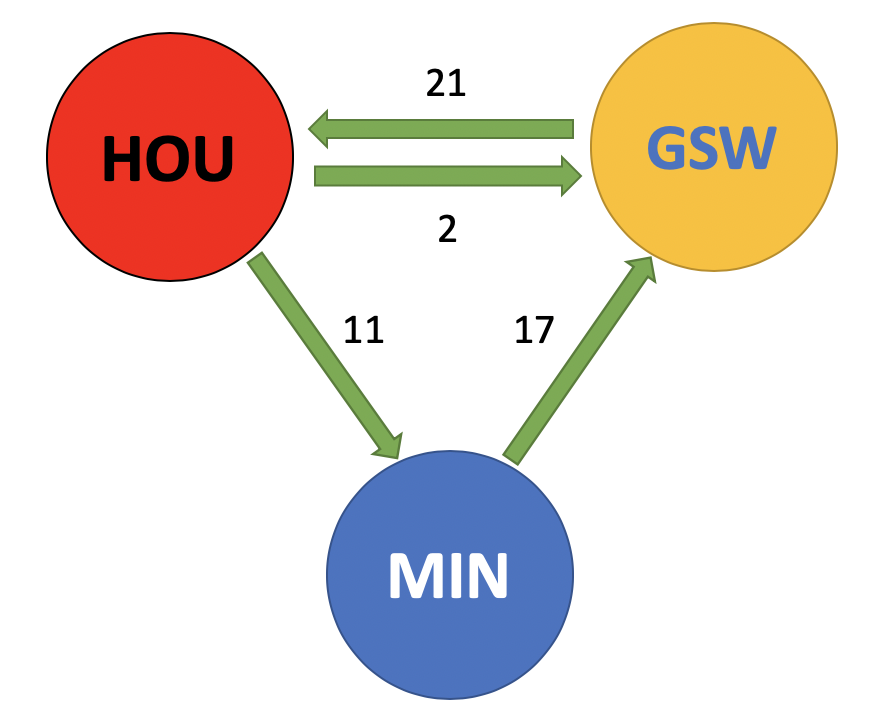
\includegraphics[width=2in]{./images/APD.png}
	\caption[Network using the APD Method]{Network using the APD Method}
\end{figure}
\begin{align*}
A_2 =\begin{bmatrix}0 & 21 & 0\\2 & 0 & 11\\17 & 0 & 0\end{bmatrix}, \textbf H_2=\begin{bmatrix}0 & 1 & 0\\0.1538 & 0 & 0.8462\\1 & 0 & 0\end{bmatrix}
\end{align*}
  
\subsubsection{Deviant Baseline (DB)}
  \null\quad\quad The DB method is a deviation from Xia and Jain's baseline method, where the directed edge is a binary indicator between teams. Using Xia and Jain's Baseline method, for entry $A_{}[i,j]$, the value is $1$ if team $j$ beat team $i$ at some point in the history of all games and $0$ otherwise. Intuitively, this is a weak network because stronger teams that repeatedly beat weaker teams should be rewarded. Therefore, we propose the DB method, which uses the total number of wins of team $j$ over team $i$. Formally,
  \[
  A_{3}[i,j]=
  \begin{cases}
  \sum_{N_{i\rightarrow j}}1 &\text{ $i$ lost to $j$}\\
  0 &\text{ otherwise}
  \end{cases}
  \]
  This produces the network shown in Figure 3. Notice that in this method, the point differential does not matter. The only consideration is the number of victory itself.
  \begin{figure}[H]
	\centering
	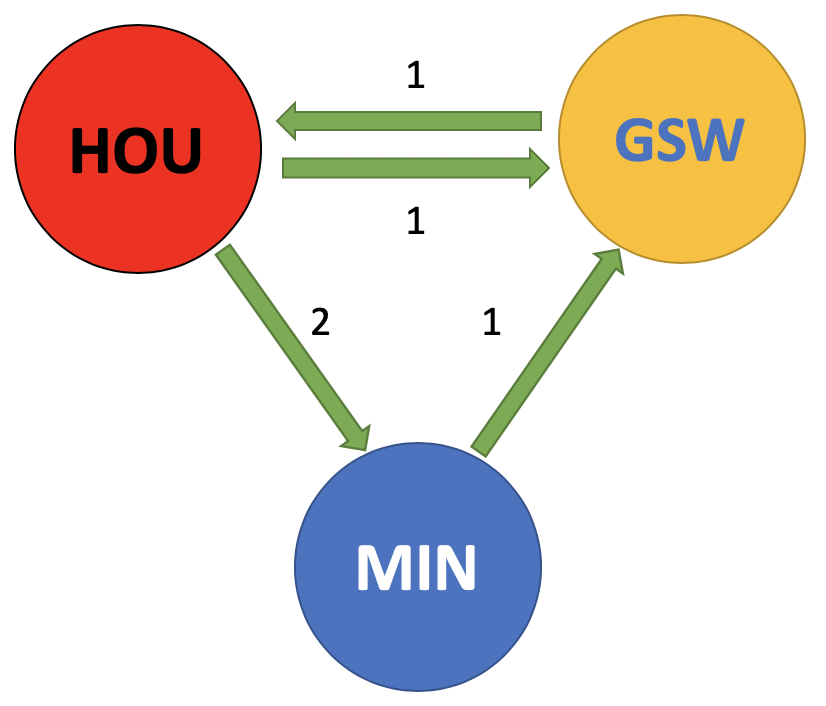
\includegraphics[width=2in]{./images/DB.png}
	\caption[Network using the DB Method]{Network using the DB Method}
\end{figure}
\begin{align*}
A_3 =\begin{bmatrix}0 & 1 & 0\\1 & 0 & 2\\1 & 0 & 0\end{bmatrix}, \textbf H_3=\begin{bmatrix}0 & 1 & 0\\0.333 & 0 & 0.667\\1 & 0 & 0\end{bmatrix}
\end{align*}

\subsubsection{Pick on Someone Your own Size (PSYS)}
  \null\quad\quad Suppose now that there is a pre-ranking of the teams, determined by their win-loss record. Unlike the previous three methods described, this is a post-processing method. It takes pre-existing team rankings and hopes to improve it by going through a second pass. Taking the existing ranking, PSYS method creates a network which greatly rewards wins of low-rank teams over high-rank teams and rewards lightly on wins of high-rank teams over low-rank teams. The intuition here is that a highly ranked team will not benefit from continually defeating poorly performing teams. Formally, suppose that there is a rank vector $\textbf{r}$, $r_a$ is the rank of team $a$, and there are $T$ total teams. If $r_i > r_j$, then team $i$ is ranked lower than rank $j$, vice versa. Then each of the entries are
  \[
  A_{4}[i,j]=
  \begin{cases}
  \Big(1-\Big(\frac{r_i-r_j}{T}\Big)^2\Big)\sum_{N_{i\rightarrow j}}1 &\text{ $i$ lost to $j$, }r_i > r_j\\
  \Big(1+\Big(\frac{r_i-r_j}{T}\Big)^2\Big)\sum_{N_{i\rightarrow j}}1 &\text{ $i$ lost to $j$, }r_i < r_j\\
  0 &\text{ otherwise}
  \end{cases}
  \]
  Parsing the notation a bit: $\Big(\frac{r_i-r_j}{T}\Big)^2$ takes the difference of the ranking of two teams and makes it a sqaured proportion (squared to ensure that it is positive). If the winning team was ranked higher, then the reward for winning is scaled down by factor $\Big(1-\Big(\frac{r_i-r_j}{T}\Big)^2\Big)\le1$. On the other hand, if the winning team was ranked lower, then the reward for winning the game is scaled up by factor $\Big(1+\Big(\frac{r_i-r_j}{T}\Big)^2\Big)\ge1$. These two scaling terms are called the rank factor, $f_r$. Notice how in this case, we use the number of wins (denoted as $\sum_{N_{i\rightarrow j}}1$), rather than point differential. If we use point differential, then we would just sum up the total point differentials, $d_{ij}$, much like in the Weighted Case (Section 2.2.1), and apply the rank factor. For this project, we use both methods of PSYS. PSYS-1 is used to denote the method using the number of wins (as shown above) and PSYS-2 is used to denote the method using point differentials.\\
  \null\quad\quad Given the example, the win loss records of each of the teams are: Golden State Warriors have a record of $2-1$, Houston Rockets have a record of $1-3$, and Minnesota Timberwolves have a record of $2-1$. Since the Timberwolves lost to the Warriors, the ranking becomes: Warriors are 1st, Timberwolves are 2nd, and Rockets are 3rd. This means that $\textbf{r}=(1,3,2)$. We run through the PSYS-1 calculation for Timberwolves versus Rockets as an example:\\
  \null\quad\quad Since the Timberwolves never lost to the Rockets, we only consider the matrix entry $A_4[1,2]$ (recall that the matrix entry is zero-indexed, team $0$ being Warriors, team $1$ being Rockets, and team $2$ being Timberwolves). Since the Rockets are ranked lower, meaning $r_1>r_2$, the first case applies. The rank factor $f_r=1-(\frac{1}{3})^2=\frac{8}{9}$. Since there are two wins, the entry $A_4[1,2]=\frac{16}{9}\approx 1.778$. We extend this for all matrix entries and for PSYS-2 to get the following networks (Figure 4) and matrices:
  \begin{figure}[H]
  \centering
\begin{subfigure}{.5\textwidth}
  \centering
  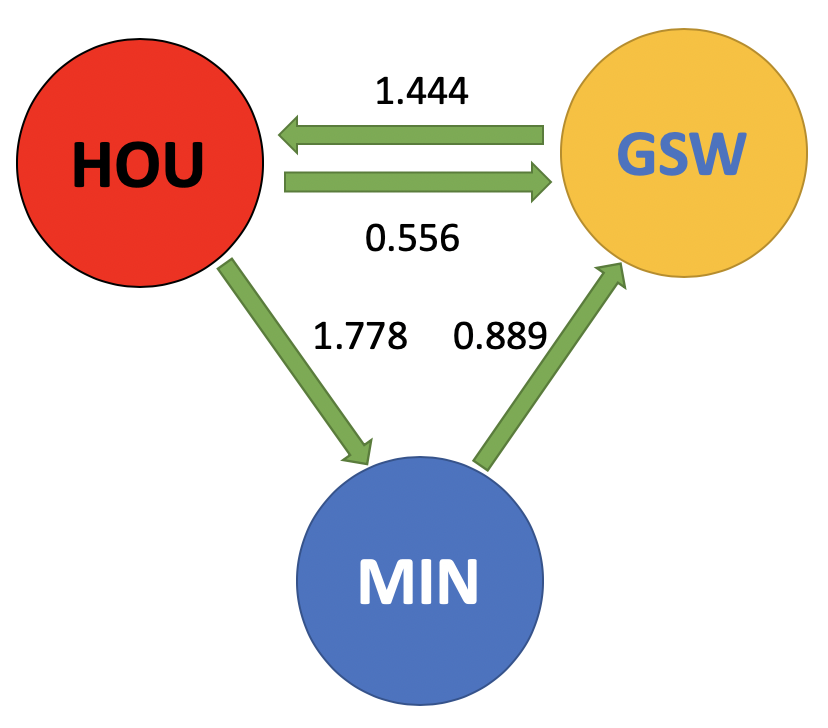
\includegraphics[width=2in]{./images/PSYS-1.png}
  \caption{Network using PSYS-1}
  \label{fig:sub1}
\end{subfigure}%
\begin{subfigure}{.5\textwidth}
  \centering
  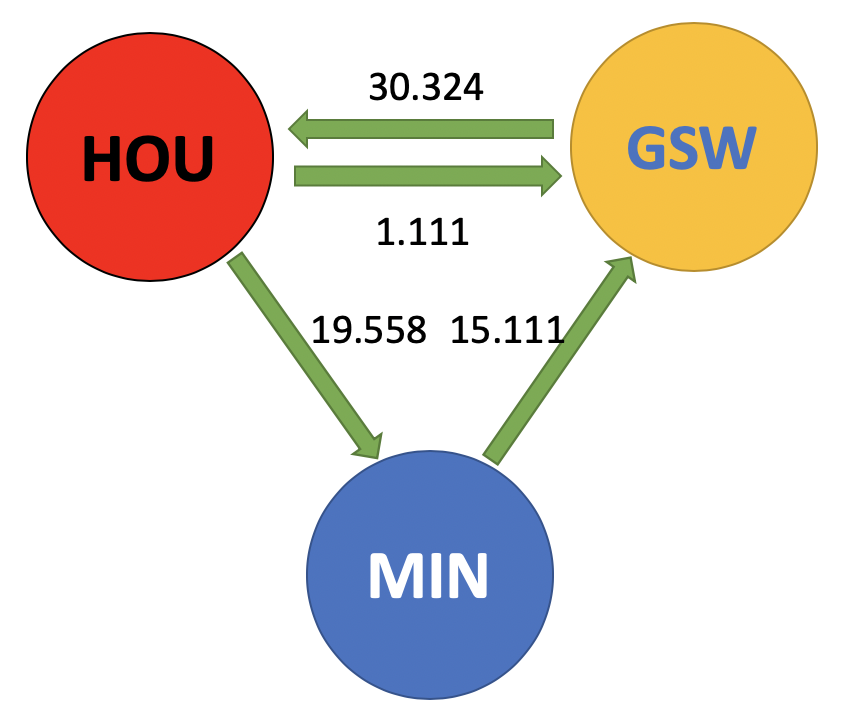
\includegraphics[width=2in]{./images/PSYS-2.png}
  \caption{Network using PSYS-2}
  \label{fig:sub2}
\end{subfigure}
\caption{Networks created using PSYS method}
\label{fig:test}
  \end{figure}
  \begin{align*}
&A_{4,1} =\begin{bmatrix}0 & 1.444 & 0\\0.556 & 0 & 1.778\\0.889 & 0 & 0\end{bmatrix}, \textbf H_{4,1}=\begin{bmatrix}0 & 1 & 0\\0.238 & 0 & 0.762\\1 & 0 & 0\end{bmatrix}\\
&A_{4,2} =\begin{bmatrix}0 & 30.324 & 0\\1.111 & 0 & 19.558\\15.111 & 0 & 0\end{bmatrix}, \textbf H_{4,2}=\begin{bmatrix}0 & 1 & 0\\0.054 & 0 & 0.946\\1 & 0 & 0\end{bmatrix}
\end{align*}

\subsection{Player Ranking Networks}
\null\quad\quad A player's performances against other players was studied using networks and the PageRank algorithm. The analysis for player ranking is further divided into team-pair analysis (Section 2.3.1) and All-Star analysis (Section 2.3.2). Both of these networks determine the ranking of players, but team-pair focuses on player performance against specific teams and All-Star generalizes for all players in the NBA. The exact implementation is discussed in Section \ref{playerimp_networks}.
\subsubsection{Team-pair Analysis}
\null\quad\quad While there are prior studies on team performances using networks, there are very limited studies on player performance using networks. Player performance was studied by pairing teams together and analyzing players' +/- metric. The +/- metric is a rating on the overall contribution of the player against specific teams. Suppose there is player $A$. If player $A$ has a high positive +/- rating against team $X$, then player $A$ plays incredibly well against team $X$. On the other hand, if player $A$ has a low negative +/- rating against team $Y$, then player $A$ plays incredibly poorly against team $Y$.\\
\null\quad\quad The adjacency matrix for the PageRank network of pairwise teams was created first by selecting two teams. Suppose there are two teams: team $X$ and team $Y$. Every single player $a\in X\cup Y$ represents a node. The adjacency matrix dimensions is given by $length(X\cup Y)$-by-$length(X\cup Y)$. For every single player $a\in X\cup Y$, the +/- rating is modified. The details for the modification is left in the Python code itself in the Appendix. The general intuition is that the +/- is scaled by a factor $p$, which is the square of the proportion of minutes played out of total possible minutes. For example, if there were $3$ games between $X$ and $Y$, then there was a maximum of $48\cdot3=144$ total minutes that a player was onthe court if they played for the entire time ($48$ minutes per game). If player $x\in X$ played for $36$ minutes, then $p=(\frac{36}{144})^2$. Though there were many other intricacies to the modification of the +/-, it has been omitted in this section. The other modifications were designed to ensure that rookies with little playing time but incredibly influential +/- ratings would not be favored over veteran players who have played consistently, more frequently.\\
\null\quad\quad Using modified +/- rating, every player in $x\in X$ is compared to player $y\in Y$. Take the difference between the two modified +/- ratings of the players. Suppose that $f(z)$ returns the modified +/- of player $z$ and define the difference to be $f(x)-f(y)$ Then we formalize the adjacency matrix as follows
\begin{align*}
A_p[x,y]=\begin{cases}
f(x)-f(y)&\text{ if }f(x)-f(y)<0\\
0 &\text{ otherwise}
\end{cases}
\end{align*}
Meaning, if player $x$ has a higher modified +/-, then there is a directed edge going from $y$ to $x$ with edge weight of the positive differential of the two modified +/-. Note that all edge weights will be positive in this network, much like how we defined the Weighted method in Section \ref{sec:2.2}.\\
\null\quad\quad As an example, suppose there are two teams, $X$ and $Y$ with two players each, indexed $i\in\{1,2\}$. Table 2 has the modified +/- of the four players.
\begin{center}
\captionof{table}{Example modified +/- values for two teams, each with two players}
\begin{tabular}{|c|c c c c|}
\hline
\textbf{Players} & $X_1$ & $X_2$ & $Y_1$ & $Y_2$\\
\hline
\textbf{+/-} & 10.1 & -5.6 & 3.7 & 12.2 \\
\hline
\end{tabular}
\end{center}
This results in the network shown in Figure 5. Note that the matrix is in the order of $X_1,X_2,Y_1,Y_2$ row-wise and column-wise.
  \begin{figure}[H]
	\centering
	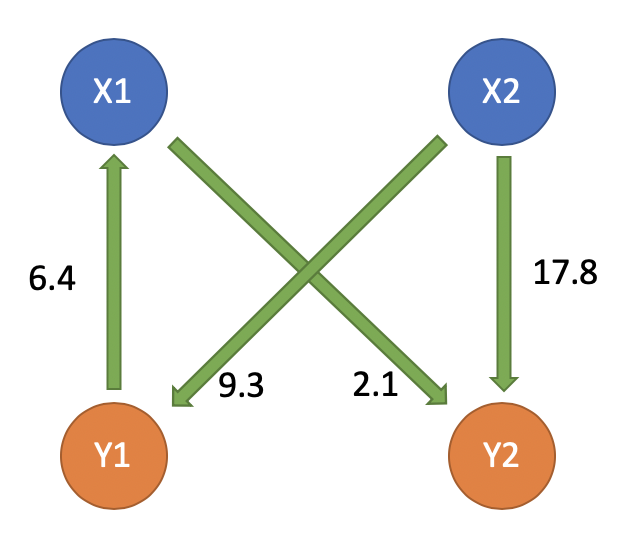
\includegraphics[width=2in]{./images/team.png}
	\caption[Network for team-pair analysis of +/-]{Network for team-pair analysis of +/-}
\end{figure}
\begin{align*}
A =\begin{bmatrix}0 & 0 & 0 & 2.1 \\0 & 0 & 9.3 & 17.8\\ 6.4 &0&0&0\\0&0&0&0\end{bmatrix}, \textbf H=\begin{bmatrix}0 & 0 & 0 & 1 \\0 & 0 & 0.343 & 0.657\\ 1 &0&0&0\\0&0&0&0\end{bmatrix}
\end{align*}
Using this team-pair analysis, the best players from each of the teams were determined from the resulting importance score rankings. For any section outside this one, modified +/- and +/- is used interchangeably to cut down on redundancy.
\subsubsection{All-Star Analysis}
\label{sec:2.3}
\null\quad\quad The All-Star analysis is generalized to study players when pit against all other players in the NBA. The exact same modified +/- differential metric was used as in the team-pair analysis above. The only difference is that the scope is the entire league. Suppose $\mathbb S$ is the set of all teams in the NBA and $X$ is one team $X\in\mathbb S$. Every single player $x\in X$ is compared to every other player $y\in \mathbb S\cap X^c$. This is repeated for every other team in $\mathbb S$. Using this network, the best players of every team, the best players in the league, the best players in the eastern conference, and the best players in the western conference were determined from the importance score ranking.
\section{Solution Implementation}
\label{implementation}
Note that all Python code and data files are available on \href{https://github.com/dchaebae/NBAPredictions}{GitHub}.
\subsection{Team Ranking Implementation}
\label{teamimp}
\subsubsection{Scraping}
\label{teamimp_scraping}
\null\quad\quad The match history of every single NBA game in the 2018-19 season were scraped using Python BeautifulSoup package from \href{https://www.basketball-reference.com/}{Basketball-Reference.com}. The files were separated out by month, meaning there is data ranging from October 2018 to May 2019. This data would primarily be used for the team analysis, as it indicates the full team names of the visiting and home teams. It also indicates the total points scored by each of the teams. A ``win'' is defined to be the team that has more points (calculated by a simple subtraction and sign check). In order to cut down on the runtime, instead of using the full team name, their 3 letter designations were used. This data was scraped from a table that contained the win/loss of a single team against every other team for all teams (conveniently had the 3 letter designations associated with the full name of the team). Python dictionaries converted to and from the 3 letter designation and the full team name. All of the data was manipulated, labeled, and stored as csv files. Consult the Appendix for more detail to scraping.
\subsubsection{Networks}
\label{teamimp_networks}
\null\quad\quad Using pandas, the csv files were read in. Numerical data were converted into NumPy matrices for easy manipulation. The adjacency matrices were created for weighted, APD, and DB methods described in Section \ref{sec:2}, and PageRank was used to get $3$ rankings of the teams. These results were compared to NBA standings, which is a ranking based simply on the number of wins and losses, without any network relations of the wins and losses. Therefore, we have 4 total rankings. These $4$ rankings were then post-processed using both PSYS-1 and PSYS-2. Therefore, there were $4+8=12$ total team rankings that were studied ($4$ before PSYS and $8$ from PSYS).\\
\null\quad\quad The $12$ rankings were analyzed in several ways. First, sequential accuracy testing was conducted to compare the accuracy of the different ranking models. The first $400$ NBA games were used to create $12 $adjacency matrices, which were then used to generate the $12$ rankings (in the case of the NBA standing ranking, we simply added the number of wins and used that to rank assuming only those first $400$ games had played). The $401^{\text{st}}$ game was used to test for accuracy. If a ranking correctly predicted for the outcome of the game (the winning team was ranked higher in the predictive set of rankings), then the model was awarded $1$ point. The $401^{\text{st}}$ game was then added to the running ``training set''. The process then repeated for initializing rankings using $401$ NBA games and testing on the $402^{\text{nd}}$ game, and so on. This test-then-add-to-training-set sequential process was done for all the non-playoff games. In total, there were $1230$ non-playoff games. Therefore, the process described above was repeated $1230-400=830$ iterations. At the end of the sequential process, the accumulated points for each of the different models were then made into proportions by dividing $830$, the total number of iterations. This is summarized in the next section, Section \ref{rnd}.\\
\null\quad\quad Next, we generated the $12$ rankings using all the non-playoff games. These rankings would then be used to predict the outcome of the playoff match-ups. Up to the end of Deans Date, there have been a total of $12$ completed match-ups. For every match-up, $1$ point was awarded if the ranking model ranked the advancing team higher than the team that lost. This analysis would be used extensively to indicate network predictive strength.\\
\null\quad\quad Lastly, we used intuitive knowledge of the game and various statistics found on \href{https://www.basketball-reference.com/}{Basketball-Reference.com} to make qualitative and quantitative assessments on the performance of the networks.

\subsection{Player Ranking Implementation}
\label{playerimp}
\subsubsection{Scraping}
\label{playerimp_scraping}
\null\quad\quad The scraping for the player ranking analysis was done completely separate from the team ranking analysis. Using BeautifulSoup, the url to each of the team roster pages were determined. For every single player on the team, their +/- rating against every other team was scraped. This was repeated for every team in the NBA (there are $30$ NBA teams and $497$ total players). Dictionaries were created to associated every player to a team index, which was then associated to a 3 letter designation by another dictionary. This dictionary sequence would be used to determine player team affiliation when creating networks.

\subsubsection{Networks}
\label{playerimp_networks}
\null\quad\quad The team-pair analysis was modularized such that using a textfile, team match-ups could be specified. PageRank was conducted using the modified +/- for all players invovled in a match-up. For instance, when looking at the Golden State Warriors (GSW) and Houston Rockets (HOU) match-up, all players from both of the teams were put into the network. Using the scheme specified in Section \ref{sec:2.3}, PageRank was conducted on the resulting adjacency matrices. Using Python, the top $5$ players from each team were determined. Similarly for the All-Star analysis, one massive network containing all the players was created using the scheme in Section \ref{sec:2.3}.\\
\null\quad\quad Given the extreme complexity of the player network and the limitation of the NBA dataset, analysis was conducted primarily on the ranking of the players. The feasibility of the network to generate the top $3$ players of every team, top $10$ players of the NBA league, top $10$ players of the Eastern Conference, and the top $10$ players of the Western Conference was studied using general knowledge of basketball and various statistics available on \href{https://www.basketball-reference.com/}{Basketball-Reference.com}. There is tremendous amount of potential, however, with this network that was created for this project. The possibilities are discussed in Section \ref{fw}, Future Work.

\section{Results and Discussion}
\label{rnd}
\subsection{Team Ranking Analysis}
\subsubsection{Sequential Accuracy Analysis}
\null\quad\quad Using the scheme discussed in Section \ref{teamimp_networks}, the following proportion accuracy graph was generated using only non-playoff data (Figure 6). It features all $12$ different ranking models and their accuracies with more training and testing. We chose to start the first iteration with $400$ games used to train the predictive model because we wanted sufficient number of games such that every team would have played every other team at least once.
\begin{figure}[H]
  \centering
  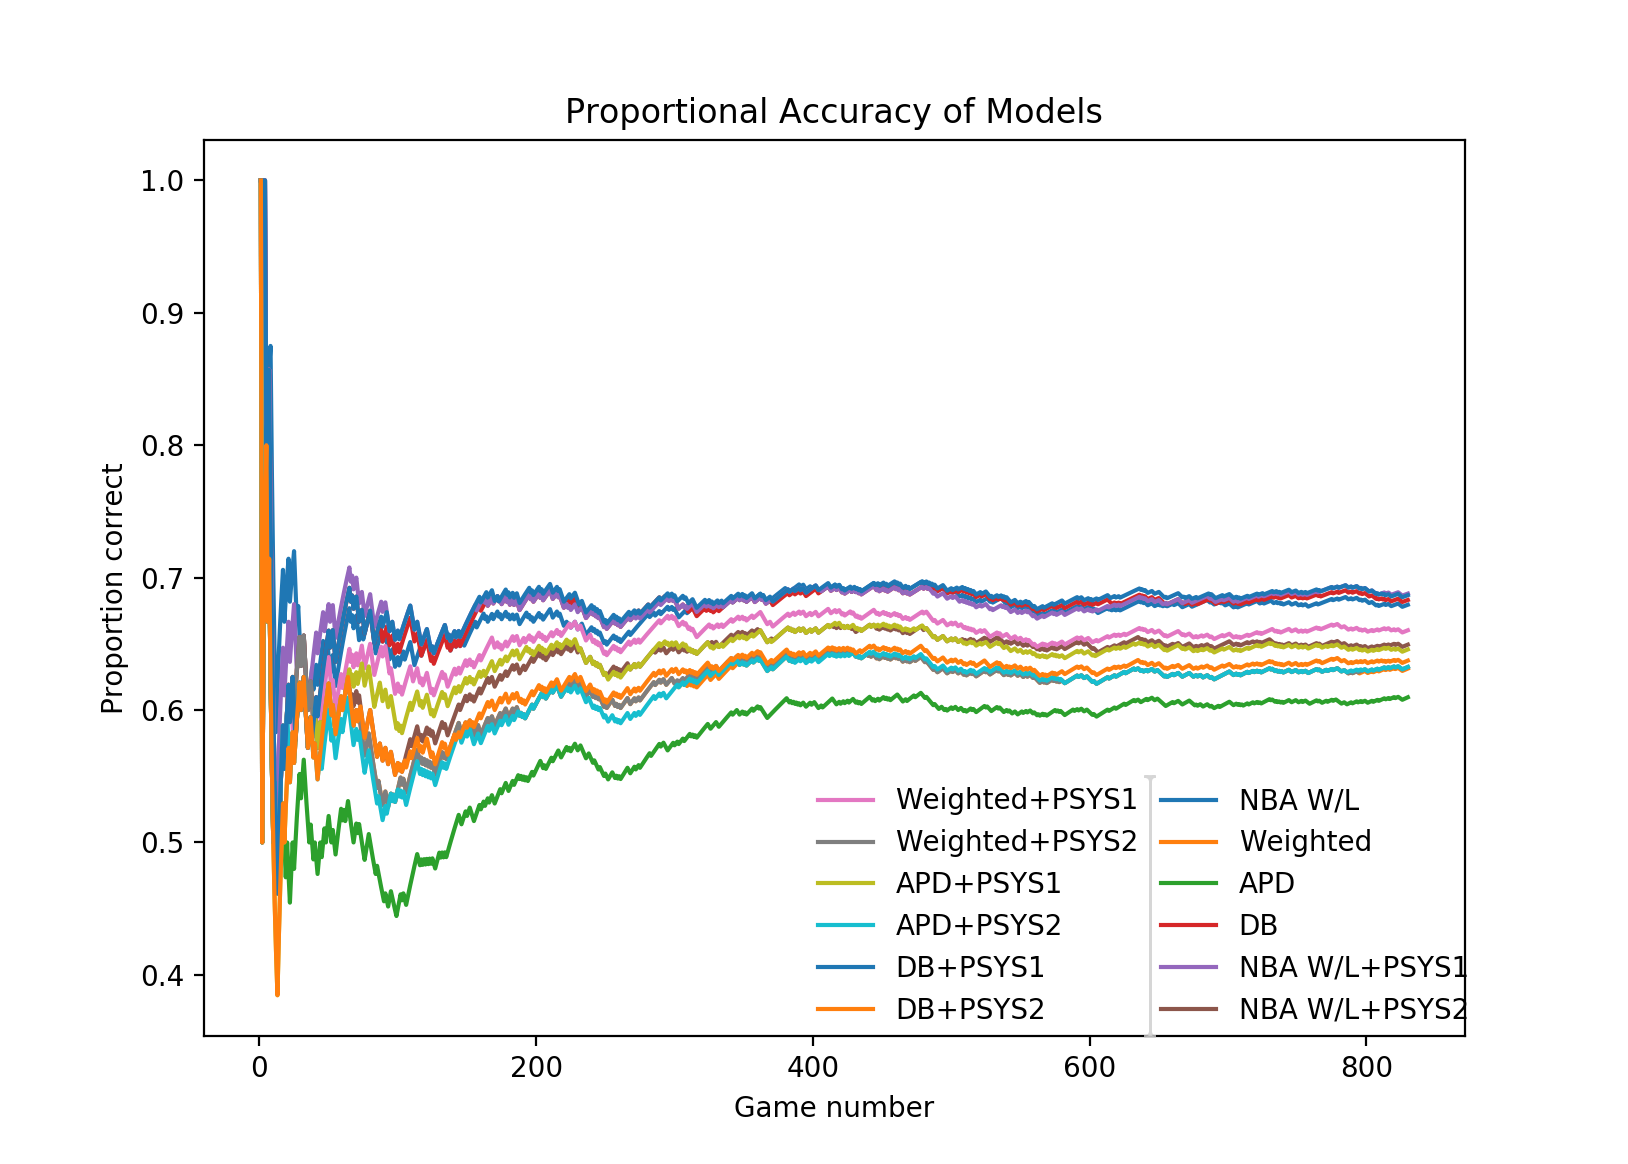
\includegraphics[width=6in]{./images/prop_acc.png}
  \caption[Proportion accuracy of the 12 ranking models]{Proportion accuracy of the 12 ranking models}
\end{figure}
Looking at the graph, all the models converged to between $0.6$ and $0.7$. This convergence was attained after approximately using $800$ games to come up with rankings ($400$ comes from starting at $400$ and around game number $400$, there is convergence, so there were $800$ training games at game number $400$). In the future, similar works should look to using at least $800$ games to reach accuracy convergence of the networks. After completing the sequential process, the final accuracies throughout the whole process for every model are shown below (Table 3).
\begin{center}
\captionof{table}{Final accuracies}
\begin{tabular}{|c c|c c|}
\hline
\textbf{Model} & \textbf{Accuracy} & \textbf{Model} & \textbf{Accuracy}\\\hline
NBA W/L&0.679&Weighted&0.631\\\hline
APD&0.610&DB&0.683\\\hline
NBA+PSYS-1&0.688&NBA+PSYS-2&0.649\\\hline
Weighted+PSYS-1&0.660&Weighted+PSYS-2&0.633\\\hline
APD+PSYS-1&0.646&APD+PSYS-2&0.633\\\hline
DB+PSYS-1&0.687&DB+PSYS-2&0.637\\\hline
\end{tabular}
\end{center}
Based on these numbers, NBA win/loss with PSYS-1 post-processing performed the best, with accuracy of $0.688$. DB+PSYS-1 and DB closely follow with accuracies $0.687$ and $0.683$ respectively. All three of these accuracies are at least $2\%$ improvements from the accuracies reported in Xia and Jain \cite{XJ}. This indicates that post-processing with the PSYS-1 network improves the accuracy of the predicted rankings. In the case of NBA standings, PSYS-1 improved the accuracy by almost $0.01$. Furthermore, using DB hold promise for predicting the outcomes of non-playoff games. With that being said, APD models predicted the worst, with PSYS-2 seemingly making networks perform worse.
\subsubsection{Playoff Analysis}
\null\quad\quad Using the entire non-playoff games to compute the rankings of the $12$ models, we analyzed the number of playoff series matchups that were predicted correctly. Up to Deans Date, there have been $12$ total matches and the number of correctly predicted advancements (defined in Solution Implementation section, Section \ref{teamimp_networks}) are shown (Table 4).
\begin{center}
\captionof{table}{Playoff series advancement accuracies}
\begin{tabular}{|c c|c c|}
\hline
\textbf{Model} & \textbf{Accuracy} & \textbf{Model} & \textbf{Accuracy}\\\hline
NBA W/L&11&Weighted&9\\\hline
APD&8&DB&10\\\hline
NBA+PSYS-1&11&NBA+PSYS-2&10\\\hline
Weighted+PSYS-1&12&Weighted+PSYS-2&9\\\hline
APD+PSYS-1&9&APD+PSYS-2&9\\\hline
DB+PSYS-1&9&DB+PSYS-2&10\\\hline
\end{tabular}
\end{center}
This time, the weighted ranking that has been post-processed by PSYS-1 (weighted+PSYS-1) performed the best, correctly predicting all $12$ playoff series matchups. The standard NBA standings- both not processed by PSYS-1 and processed by PSYS-1 - come in close with $11$ correct predictions. All other network models have at least $2$ incorrect predictions of the playoffs. Therefore, it seems to be that weighted+PSYS-1 best predicts playoff results. This is a different model from the models that performed the best in the previous section. This may be accounted because players tend to try harder in hopes of advancing in the playoff series, whereas for regular season matches, the level of seriousness is a bit lower.
\subsubsection{Qualitative Rank Analysis}
\null\quad\quad We ranked the 30 teams using the weighted, APD, DB methods (code shown in Appendix A.2 and the rankings of the PSYS models are shown in Appendix B), in comparison to the standard NBA standing rankings (Table 5). The ranking of the teams are shown below. The raw importance vectors for each of the different methods are shown in Appendix B.
\begin{center}
\captionof{table}{Team rankings using weighted, APD, and DB methods}
\begin{tabular}{|c|c |c |c| c|}
\hline
\textbf{Team} & \textbf{Weighted Rank} & \textbf{APD Rank} & \textbf{DB Rank} & \textbf{NBA Standings}\\
\hline
Atlanta Hawks & 28& 27& 26&26\\\hline
Boston Celtics &13 &15 &12&9 \\\hline
Brooklyn Nets & 19& 20&15 &14\\\hline
Chicago Bulls & 29& 29& 29&27\\\hline
Charlotte Hornets & 22& 24&21&18 \\\hline
Cleveland Cavaliers &26 & 25& 28&28 \\\hline
Dallas Mavericks & 15&12 &20&24 \\\hline
Denver Nuggets & 10& 13&4&4 \\\hline
Detroit Pistons & 23& 21&17&16 \\\hline
Golden State Warriors & 2& 3&3&3 \\\hline
Houston Rockets & 5&8 &2&5 \\\hline
Indiana Pacers & 7& 2& 14&12\\\hline
Los Angeles Clippers &14 & 14&11& 13\\\hline
Los Angeles Lakers & 17& 18&19&20 \\\hline
Memphis Grizzlies & 21& 23&16&22 \\\hline
Miami Heat & 16& 16&18&17 \\\hline
Milwaukee Bucks & 1& 1& 1&1\\\hline
Minnesota Timberwolves & 18& 19&22&21 \\\hline
New Orleans Pelicans & 20& 22&24&23 \\\hline
New York Knicks & 30& 30& 30&30\\\hline
Oklahoma City Thunder &9 &9 &6&10 \\\hline
Orlando Magic & 11&11 &13 &15\\\hline
Philadelphia 76ers &12 &6 &10&7 \\\hline
Phoenix Suns & 27& 28& 27&29\\\hline
Portland Trail Blazers  &4 &7 &5&6 \\\hline
Sacramento Kings & 25&26 &23&19 \\\hline
San Antonio Spurs & 6& 4&8& 11\\\hline
Toronto Raptors & 8& 10&7&2 \\\hline
Utah Jazz &3 & 5& 9 &8\\\hline
Washington Wizards & 24& 17& 25 &25 \\\hline
\end{tabular}
\end{center}
\null\quad\quad Using the APD method, the Indiana Pacers were notably higher than anticipated. In analyzing the process for assigning weights, we realized that the Pacers have had relatively large wins against teams that they do not play very often, like the Los Angeles Lakers. The Pacers defeated the Lakers by $42$ points in one game and lost by $8$ in the next game between the two. In both the weighted method and APD, this results in a link from Lakers to the Pacers with weight $42$ and a link from the Pacers to the Lakers with weight $8$. In the weighted model, this did not really cause an issue because there were many links with weights greater than $40$. However, in the APD, teams rarely had a blowout with the same team twice, so there were not many links with weights greater than approximately $25$. Thus the APD favored teams like the Pacers over teams that may have more consistent winning records with smaller win margins. These effects are observed on the APD because there are insufficient number of games played for a given team match-up. If there were more games, then it may be possible that APD performs better. We considered combining previous seasons, but that would introduce variables that would be difficult to control, e.g. players changing teams.\\
\null\quad\quad Of the three rankings, the DB method best matched our expectations. In the NBA, there are a relatively large number of total games, but each team may only play a particular opponent a few times in a season. Because of this and characteristics of the model, a team that was inconsistent, but had wins by larger margins, like the Pacers, was favored over teams that won more consistently by smaller margins. Consider the case of the Toronto Raptors, who had the second-best record in the entire league, but were ranked eighth and tenth using the weighted and APD methods, respectively. In both cases, the Raptors have actually beaten all but two of the teams ranked above them. The DB method offers an alternative to the weighted and APD methods in that wins are each valued the same. ``A win is a win'' as they say, and sometimes it does not matter how you secure it. When we later use test data, it will be interesting to see which model performs better in prediction and whether or not our intuition was correct.\\

\subsection{Player Ranking Analysis}
\subsubsection{Team-pair Analysis}
\null\quad\quad Creating a network between individual players was beneficial in considering specific match-ups between teams, which we achieved by selecting specific pairs from the $30$ teams and replicating the general network strategy within each pairing, using the games exclusively between those two teams throughout the season. In total there are $435$ differnet pair combinations of teams (30 choose 2). While we cannot conduct a thorough analysis of each of the $435$ networks, we have included examples of the two upcoming series in this season's playoffs and two examples of recently completed playoffs series.

\begin{center}
\captionof{table}{Golden State Warriors (GSW) versus Portland Trail Blazers (POR) upcoming match-up}
\begin{tabular}{|c|c c c|}
\hline
\textbf{Rank} &\textbf{Top 5 from GSW} &\textbf{Top 5 from POR}&\textbf{Top 5 from match-up}\\\hline
1&Draymond Green&Rodney Hood&Rodney Hood\\\hline
2&Andre Iguodala&Damian Lillard&Draymond Green\\\hline
3&Kevin Durant&CJ McCollum&Andre Iguodala\\\hline
4&Jonas Jerebko&Jusuf Nurkic&Kevin Durant\\\hline
5&Klay Thompson&Al-Farouq Aminu&Jonas Jerebko\\\hline
\end{tabular}
\end{center}
\begin{center}
\captionof{table}{Golden State Warriors (GSW) versus Houston Rockets (HOU) completed match-up}
\begin{tabular}{|c|c c c|}
\hline
\textbf{Rank} &\textbf{Top 5 from GSW} &\textbf{Top 5 from HOU}&\textbf{Top 5 from match-up}\\\hline
1&Damian Jones&Eric Gordon&Damian Jones\\\hline
2&Andre Iguodala&James Harden&Eric Gordon\\\hline
3&Kevin Durant&Clint Capela&James Harden\\\hline
4&Stephen Curry&Danuel House&Clint Capela\\\hline
5&DeMarcus Cousins&P.J. Tucker&Danuel House\\\hline
\end{tabular}
\end{center}

\begin{center}
\captionof{table}{Toronto Raptors (TOR) versus Milwaukee Bucks (MIL) upcoming match-up}
\begin{tabular}{|c|c c c|}
\hline
\textbf{Rank} &\textbf{Top 5 from TOR} &\textbf{Top 5 from MIL}&\textbf{Top 5 from match-up}\\\hline
1&Kawhi Leonard&Malcolm Brogdon&Malcolm Brogdon\\\hline
2&Serge Ibaka&Giannis Antetokounmpo&Kawhi Leonard\\\hline
3&Fred VanVleet&Donte DiVincenzo&Serge Ibaka\\\hline
4&Danny Green&Khris Middleton&Fred VanVleet\\\hline
5&Kyle Lowry&Eric Bledsoe&Giannis Antetokounmpo\\\hline
\end{tabular}
\end{center}

\begin{center}
\captionof{table}{Toronto Raptors (TOR) versus Philadelphia 76ers (PHI) completed match-up}
\begin{tabular}{|c|c c c|}
\hline
\textbf{Rank} &\textbf{Top 5 from TOR} &\textbf{Top 5 from PHI}&\textbf{Top 5 from match-up}\\\hline
1&Serge Ibaka&James Ennis&Serge Ibaka\\\hline
2&Kyle Lowry&T.J. McConnell&Kyle Lowry\\\hline
3&Kawhi Leonard&J.J. Redick&Kawhi Leonard\\\hline
4&Danny Green&Ben Simmons&Danny Green\\\hline
5&Pascal Siakam&Mike Scott&Pascal Siakam\\\hline
\end{tabular}
\end{center}
\null\quad\quad While these lists largely contain similar names from our larger league-wide analysis and many other well-known players (discussed in Section \ref{allstaranalysis}, the All-Star Analysis Section), the benefit of these networks lie in understanding what has previously worked or failed in earlier games from match-ups and using that to gameplan for the next upcoming games. For example, in looking at the upcoming series between the Golden State Warriors (GSW) and the Portland Trail Blazers (POR), we can see the significant lack of Stephen Curry, who was indicated as being the best player on the Warriors by our league-wide model (Section \ref{allstaranalysis}), and the inclusion of Andre Iguodala, Jonas Jerebko, and Klay Thompson. A closer look shows that Curry has struggled against the Trail Blazers, relative to other opponents, by multiple metrics including, but not limited to +/-. The players that were listed for the Warriors also notably play largely from the wing, as opposed to the top of the key or the low-post. By also looking at the players listed for the Trail Blazers, it seems as though the Warriors had a favorable advantage in this area of the court. Indeed, the Trail Blazers are known for primarily for their backcourt guards, CJ McCollum and Damian Lillard, and their inside bigs. While they may be relatively vulnerable on the wings, they should look to rely on their three-point shooting and exploit their advantage on the offensive and defensive rebounds. However, these strategies are changed, especially for Golden State, due to the recent injury and expected absence of Kevin Durant, an undeniable focal point of the team.\\
\null\quad\quad In their previous series against the Houston Rockets, the Golden State Warriors had a different top five that included rookie Damian Jones and superstar DeMarcus Cousins. Both players are $7$-foot-tall centers that control the area closest to the basket. The Rockets relied heavily on their $6$-foot-$10$ center Clint Capela as a large piece of their offense. The increase in the importance of both Jones and Cousins in this series came from the relative match-up against Capela. Typically, Golden State plays $6$-foot-$7$ Draymond Green in that position, but the height difference had proven to be too great of a factor in previous games. Unfortunately, the Warriors did not have the option of executing this strategy as both Jones and Cousins were injured and ineligible to play prior to the start of the series.\\
\null\quad\quad On the other side of the bracket, we can look to the upcoming series between the Milwaukee Bucks (MIL) and the Toronto Raptors (TOR). Milwaukee's best five in this match-up include Giannis Antetokounmpo, the best overall player in the league, according to our prior application, and an abundance of players who can shoot $3$-pointers in Malcolm Brogdon, Donte DiVincenzo, and Khris Middleton. Antetokounmpo, who excels at driving towards the basket and drawing the defense towards him, should either look to finish with a shot close to the basket or passing it to one of his teammates on the outside for an open $3$-pointer. This strategy worked well for them in their previous series, and no one has really found a solution to it yet. Eric Bledsoe, a point guard who can also handle the ball, is necessary to relieve the pressure of Antetokounmpo having the ball on every play. In response, Toronto will also have to rely more on its own 3-point shooters, Fred VanVleet and Danny Green, and less on players like Pascal Siakam, who would be disadvantaged in an individual match-up against Antetokounmpo, in order to stay close throughout the game. 

\subsubsection{All-Star Analysis}
\label{allstaranalysis}
\null\quad\quad The player network that we created consists of every current NBA player and considers their performance against every other team in the league across the entirety of the $82$-game season via the modified +/- score. From that network, we produced a ranked list of all individual players, which were then divided by conference and by team. The rankings are shown in the Tables below
\begin{center}
\captionof{table}{Top 10 players in the NBA, Eastern Conference, and Western Conference}
\begin{tabular}{|c|c c c|}
\hline
\textbf{Rank} &\textbf{NBA} &\textbf{Eastern Conference}&\textbf{Western Conference}\\\hline
1 & Giannis Antetokounmpo & Giannis Antetokounmpo & Paul George\\\hline
2&Paul George & Malcolm Brogdon & Stephen Curry\\\hline
3&Malcolm Brogdon & Kawhi Leonard & Draymond Green\\\hline
4&Kawhi Leonard&  Kyle Lowry & Kevin Durant\\\hline
5&Kyle Lowry & Khris Middleton & Damian Lillard\\\hline
6&Khris Middleton & Pascal Siakam&Ruby Gobert\\\hline
7&Pascal Siakam & Danny Green&David Bertans\\\hline
8&Stephen Curry & Brook Lopez&Nikola Jokic\\\hline
9&Danny Green & Eric Bledsoe&Jamal Murray\\\hline
10&Brook Lopez & Al Horford&Dennis Schroder\\\hline
\end{tabular}
\end{center}

\begin{center}
\captionof{table}{Top 3 players for every team}
\begin{tabular}{|c|c c c|}
\hline
\textbf{Team} & \textbf{Rank 1} & \textbf{Rank 2} & \textbf{Rank 3}\\
\hline
Atlanta Hawks &John Collins&Kevin Huerter&Taurean Prince\\\hline
Boston Celtics &Al Horford&Jayson Tatum&Kyrie Irving\\\hline
Brooklyn Nets &DeMarre Carroll&D'Angelo Russell&Joe Harris\\\hline
Chicago Bulls &Ryan Arcidiacono&Lauri Markkanen&Otto Porter\\\hline
Charlotte Hornets &Nicolas Batum&Kemba Walker&Jeremy Lamb\\\hline
Cleveland Cavaliers &David Nwaba&Tristan Thompson&Brandon Knight\\\hline
Dallas Mavericks &Dwight Powell&Dorian Finney-Smith&Luka Doncic\\\hline
Denver Nuggets &Nikola Jokic&Jamal Murray&Paul Millsap\\\hline
Detroit Pistons &Andre Drummond&Langston Galloway&Luke Kennard\\\hline
Golden State Warriors &Stephen Curry&Draymond Green&Kevin Durant\\\hline
Houston Rockets &James Harden&Clint Capela&Chris Paul\\\hline
Indiana Pacers &Domantas Sabonis&Cory Joseph&Myles Turner\\\hline
Los Angeles Clippers &Lou Williams&Patrick Beverley&Danilo Gallinari\\\hline
Los Angeles Lakers &LeBron James&Lonzo Ball&Josh Hart\\\hline
Memphis Grizzlies &Mike Conley&Jonas Valanciunas&Jaren Jackson Jr.\\\hline
Miami Heat &Justise Winslow&Josh Richardson&Hassan Whiteside\\\hline
Milwaukee Bucks&Giannis Antetokounmpo&Malcolm Brogdon&Khris Middleton\\\hline
Minnesota Timberwolves &Jeff Teague&Robert Covington&Taj Gibson\\\hline
New Orleans Pelicans &Jrue Holiday&Anthony Davis&E'Twaun Moore\\\hline
New York Knicks &Dennis Smith Jr.&Noah Vonleh&Damyean Dotson\\\hline
Oklahoma City Thunder &Paul George&Dennis Schroder&Jerami Grant\\\hline
Orlando Magic & Nikola Vucevic&Evan Fournier&Aaron Gordon\\\hline
Philadelphia 76ers &Joel Embiid&J.J. Redick&Jimmy Butler\\\hline
Phoenix Suns &Kelly Oubre Jr.&Devin Booker&Deandre Ayton\\\hline
Portland Trail Blazers  &Damian Lillard&CJ McCollum&Jusuf Nurkic\\\hline
Sacramento Kings &Bogdan Bogdanovic&Buddy Hield&Willie Cauley-Stein\\\hline
San Antonio Spurs &Davis Bertans&LaMarcus Aldridge&Patty Mills\\\hline
Toronto Raptors & Kawhi Leonard&Kyle Lowry&Pascal Siakam\\\hline
Utah Jazz &Rudy Gobert&Joe Ingles&Donovan Mitchell\\\hline
Washington Wizards &Bradley Beal&Tomas Satoransky&Jeff Green\\\hline
\end{tabular}
\end{center}
\null\quad\quad While the original intent of this league-wide player analysis was to produce potential All-Star or MVP suggestions, a closer look at the rankings suggested that we may not have been as successful as we hoped. Despite the fact that all of the players listed in the overall and conference rankings performed very well this year, not all of them would intuitively qualify as MVP candidates. For example, although Malcolm Brogdon is widely considered an All-Star-caliber player, he is certainly not seriously considered to be the MVP, especially when he's not even the best player on his own team (Giannis Antetokounmpo). Looking at the overall top $10$, $4$ of the $10$ play for the Milwaukee Bucks and another $4$ of the $10$ play for the Toronto Raptors. The Bucks had the best overall record, paired with the highest team +/- rating in the league, while the Raptors had the second-best overall record, paired with the third highest +/- rating in the league. We believe that there is a carry-over effect simply by being on the better teams. Imagine two identical players, one playing the best team in the league, and the other playing for the worst team in the league. While these players may have the exact same individual impact on their teams' performances, the player on the better team will attain a high +/- simply by virtue of having better teammates, which would artificially inflate the individual's ranking in this system. It is also possible then, that this system also deflates the importance of the best player on a team that is over-represented with multiple players (Giannis Antetokounmpo and Kawhi Leonard). This corresponds to the idea that in addition to having spectacular individual performances, certain players also made the other players around them better. Unfortunately, because of the need to have unique links in our network, the +/- was the most viable metric we could use. Other stats may yield different player rankings, but do not utilize a network model to do so.\\
\null\quad\quad Fortunately, the over-representation of teams with better +/- ratings becomes irrelevant when we look at the best players within any given team. Although it may be a stretch to say that these lists establish a consensus hierarchy of skill within a team, they do provide an analytical insight as to who has a notable positive presence on the court. There were a few unexpected features worth pointing out. James Harden, the reigning MVP from last season and a strong candidate for the repeat award, stood outside the top $10$ in the Western Conference. Despite the incredible volume of his output (an astounding $36$ points per game compared to second place $28$ points per game and $650$+ total points than the nearest competitor over the course of the season), his lack of defensive impact may be reason enough for his relatively low ranking. Similarly, Russell Westbrook, the most recent MVP prior to Harden did not even rank within the top three players on his team; though, like Harden, despite the large volume of his offensive production, he has been criticized for lack of a balanced game. Finally, LeBron James, largely considered to be the best basketball player in the world, ranked very low. However, his team, the Los Angeles Lakers, simply did not perform well this season for a variety of reasons, which is associated with him having a low +/- rating.\\

\section{Conclusion}
\label{concl}
\null\quad\quad So far, there have been very few studies on the use of networks to rank sports teams and no studies on the use of networks to study the relationship between different players. In this work, we focused on the NBA dataset and proposed APD and DB networks, as well as the PSYS post-processing scheme. This study found that PSYS-1 is an incredibly powerful post-processing network that could be used as a tool to improve rankings of teams. Specifically, weighted+PSYS-1 could be used to predict playoff outcomes whereas DB+PSYS-1 or DB could be used to predict non-playoff game outcomes. In addition, there is great potential for future work with networks of players (see next section, Section \ref{fw}). Therefore, the present work supports the strong potential of networks in generating more convincing sports team rankings that rely more on the relationship between different teams than on pure individual team performance metrics such as win/loss records.

\section{Future Work}
\label{fw}
\null\quad\quad In Xia and Jain's study, they were able to factor in ``momentum wins'' by applying a $\lambda$ to scale down consecutive wins. As the relationship of this with our models was not studied, future works could consider this as a possible avenue for improving rankings via networks. \\
\null\quad\quad Another major work for the future is regards the huge potential of player data. The player data is in many ways, lacking, as there are no player statistics on a per-game basis. Having access to this data would be incredible valuable, as it would allow for more dynamic analysis of player performance against teams in specific conditions. Another possible avenue for future work could analyze player performance with positions in consideration. A point guard may play completely different roles than a forward might, which results in different player statistics. Networks could potentially be made to study the effects of different positions and actions that would be the ``best-response'' against a player of another position.

\section{Contribution of Individuals}
\null\quad\quad Daniel Chae ('20) primarily focused on the code of the project. This involved scraping the dataset, creating the adjacency matrices, and running the PageRank algorithm. Drey Tengan ('20) then used the result of the code to analyze the team rankings and the player rankings systematically. He conducted both qualitative and quantitative analysis (the proportional accuracies) to draw significant conclusions. Drey Tengan also largely contributed to the theoretical and mathematical formulation of PSYS and the modified +/- metric. Overall, the workload was fair and divided equally.

\section{References}
\printbibliography[heading=none]
\newpage
\section{Appendix}
\subsection{Appendix A.1}
Scraping code is shown below in Python. It uses BeautifulSoup, pandas, and NumPy to accomplish the task.
\noindent\hrulefill
\begin{lstlisting}[language=Python]
from urllib.request import urlopen
from bs4 import BeautifulSoup, Comment
import pandas as pd
import numpy as np

def scraper(query, year=2019):
	""" Scrape NBA data from basketball-reference.com
	"""
	for i in range(query.shape[0]):
		url = query[i,0].format(year)
		html = urlopen(url)
		soup = BeautifulSoup(html, "lxml")
		print("Generating {} using {}".format(query[i,1]\
				.format(year), query[i,2]))

		# Grab the headers
		html = None
		head = soup.find(id=query[i,2])
		head_ind = int(query[i,3]) # start of header index
		# Case 1: Check to see if delineated by comments
		for c in head.children:
			if isinstance(c, Comment):
				html = c
		if html is not None:
			soup = BeautifulSoup(html, "lxml")
			headers = [th.getText() for th in soup.\
				find_all('tr', limit=head_ind+1)\
				[head_ind].find_all('th')]
		# Case 2: Not delineated by comments
		else:
			headers = [th.getText() for th in head.\
				find_all('tr', limit=head_ind+1)\
				[head_ind].find_all('th')]
		headers = headers[1:]

		# Grab the data
		rows = soup.findAll('tr')[head_ind+1:]
		stats = [[td.getText() for td in rows[i].\
				findAll('td')]
		        for i in range(len(rows))]

		stats = pd.DataFrame(stats, columns = headers)
		stats.to_csv("./scrapedData/{}".format(\
				query[i,1].format(year)))

query = np.genfromtxt('scrape.txt', dtype='str')
scraper(query)
\end{lstlisting}
There was a text file to specify various parameters. In this case, the text file consisted of:\\
https://www.basketball-reference.com/leagues/NBA\_\{\}\_per\_game.html\\ player\_stats\_\{\}.csv per\_game\_stats 0\\
https://www.basketball-reference.com/leagues/NBA\_\{\}.html \\team\_stats\_\{\}.csv all\_team-stats-per\_game 0\\
https://www.basketball-reference.com/leagues/NBA\_\{\}.html \\opponent\_stats\_\{\}.csv all\_opponent-stats-per\_game 0\\
https://www.basketball-reference.com/leagues/NBA\_\{\}.html \\misc\_stats\_\{\}.csv all\_misc\_stats 1\\
https://www.basketball-reference.com/leagues/NBA\_\{\}.html \\team\_shooting\_\{\}.csv all\_team\_shooting 2\\
https://www.basketball-reference.com/leagues/NBA\_\{\}.html \\opponent\_shooting\_\{\}.csv all\_opponent\_shooting 2\\
https://www.basketball-reference.com/leagues/NBA\_\{\}\_standings.html\\ standings\_\{\}.csv all\_expanded\_standings 1\\
https://www.basketball-reference.com/leagues/NBA\_\{\}\_standings.html\\ teamvteam\_\{\}.csv all\_team\_vs\_team 0\\
https://www.basketball-reference.com/leagues/NBA\_\{\}\_games-october.html\\ month\_october\_\{\}.csv schedule 0\\
https://www.basketball-reference.com/leagues/NBA\_\{\}\_games-november.html\\ month\_november\_\{\}.csv schedule 0\\
https://www.basketball-reference.com/leagues/NBA\_\{\}\_games-december.html\\ month\_december\_\{\}.csv schedule 0\\
https://www.basketball-reference.com/leagues/NBA\_\{\}\_games-january.html\\ month\_january\_\{\}.csv schedule 0\\
https://www.basketball-reference.com/leagues/NBA\_\{\}\_games-february.html\\ month\_february\_\{\}.csv schedule 0\\
https://www.basketball-reference.com/leagues/NBA\_\{\}\_games-march.html\\ month\_march\_\{\}.csv schedule 0\\
https://www.basketball-reference.com/leagues/NBA\_\{\}\_games-april.html\\ month\_april\_\{\}.csv schedule 0\\
\subsection{Appendix A.2}
The Python code for running the team analysis is shown below
\begin{lstlisting}[language=Python]
import numpy as np
import pandas as pd
import glob

# Iterate through PageRank algorithm using G matrix, matrix, 
# and the initial importance vector
def converger(importance, matrix):
	while True:
		next_importance = np.matmul(importance, matrix)
		l1_dist = np.sum(abs(importance-next_importance))
		importance = next_importance
		if l1_dist < 1e-20:
			break
	return importance

# Analysis for 2019 year, can be used for other years as needed
YEAR=2019
games_month = glob.glob("./scrapedData/month*_\{\}.csv".format(YEAR))
data_month = []
# combine all the months to one Dataframe
for filename in games_month:
	df = pd.read_csv(filename)
	data_month.append(df)

df = pd.concat(data_month, ignore_index=True)
(visit_name, visit_pointcol, home_name, home_pointcol) = \
					df.columns[2:6]
# Remove games that have not yet been played (but are 
# included in scrape)
not_played_ind = np.argwhere(np.isnan(df[home_pointcol]))
not_played_ind = np.reshape(not_played_ind, \
				not_played_ind.shape[0])
df = df.drop(not_played_ind)
df.index = range(df.shape[0])
df.to_csv('./teamRank/check.csv')

# map full team name to 3 letter name to index
teamvteam_data = pd.read_csv("./scrapedData/\
			teamvteam_\{\}.csv".format(YEAR))
abbr_names = teamvteam_data.columns[2:]
full_names = teamvteam_data['Team']
num_teams = abbr_names.shape[0]
name_dict = dict(zip(full_names, abbr_names))
ind_dict = dict(zip(abbr_names, range(num_teams)))
print(ind_dict)
teamvteam_np = teamvteam_data.to_numpy()[:,2:]

# make an empty 2d NumPy array to store sums
# rowPoint-colPoint scoring system
relation_matrix = np.zeros((num_teams, num_teams))
visit_teams = df[visit_name]
visit_points = df[visit_pointcol]
home_teams = df[home_name]
home_points = df[home_pointcol]
diff_points = visit_points-home_points
for i in range(df.shape[0]):
	visit_ind = ind_dict[name_dict[visit_teams[i]]]
	home_ind = ind_dict[name_dict[home_teams[i]]]
	if diff_points[i] > 0:
		relation_matrix[visit_ind, home_ind] \
				+= diff_points[i]
	else:
		relation_matrix[home_ind, visit_ind] \
				+= abs(diff_points[i])

pd.DataFrame(relation_matrix.T).to_csv('./teamRank/sums.csv')

# Run the PageRank Algorithm but for ranking teams, use SUM!
# A replication of Xia & Jain's weighted method
normalizer = np.sum(relation_matrix.T, axis=1)
normalizer[normalizer == 0] = 1
H = relation_matrix.T /normalizer[:,None]
pd.DataFrame(H).to_csv('./teamRank/H_matrix.csv')
importance = np.ones(num_teams)/num_teams
# check for any dangling nodes
zero_indices = np.where(~H.any(axis=1))[0]
H[zero_indices,:] = importance # make H hat
pd.DataFrame(H).to_csv('./teamRank/H_hat_matrix.csv')

t = 0.85
G = t * H + (1-t)/num_teams*np.ones((num_teams, num_teams))
pd.DataFrame(G).to_csv('./teamRank/G_matrix.csv')
importance = converger(importance, G)
print('Xia & Jain\'s Weighted Method--------------------')
print('Importance vector: {}'.format(importance))
importance_rank = np.argsort(importance)[::-1]
print('Rank of teams: {}'.format(full_names.\
				to_numpy()[importance_rank]))

#----------------------------------------------------------
# Two more ways of ranking are used:
# First: take the average based on number of games (pairs)
# Second: take the total number of wins (similar to baseline
# method described in Xia and Jain, but not clamped to 0 or 1)
#----------------------------------------------------------
baseline_matrix = np.zeros((num_teams, num_teams))
for i in range(teamvteam_np.shape[0]):
	for j in range(i+1, teamvteam_np.shape[1]):
		winloss = teamvteam_np[i, j]
		winloss_split = winloss.split("-")
		if int(winloss_split[0]) > 0:
		  relation_matrix[i, j] /= int(winloss_split[0])
		  baseline_matrix[i, j] += int(winloss_split[0])
		if int(winloss_split[1]) > 0:
		  relation_matrix[j, i] /= int(winloss_split[1])
		  baseline_matrix[j, i] += int(winloss_split[1])
relation_matrix = relation_matrix.T 
baseline_matrix = baseline_matrix.T 
pd.DataFrame(relation_matrix).to_csv('./teamRank/avgs.csv')
pd.DataFrame(baseline_matrix).to_csv('./teamRank/\
				baseline_deviant.csv')

# FIRST METHOD
# Run the PageRank Algorithm but for ranking teams, use AVERAGE!
normalizer = np.sum(relation_matrix, axis=1)
normalizer[normalizer == 0] = 1
H = relation_matrix /normalizer[:,None]
pd.DataFrame(H).to_csv('./teamRank/H_matrix.csv')
importance = np.ones(num_teams)/num_teams
# check for any dangling nodes
zero_indices = np.where(~H.any(axis=1))[0] 
H[zero_indices,:] = importance # make H hat
pd.DataFrame(H).to_csv('./teamRank/H_hat_matrix.csv')
t = 0.85
G = t * H + (1-t)/num_teams*np.ones((num_teams, num_teams))
pd.DataFrame(G).to_csv('./teamRank/G_matrix.csv')
importance = converger(importance, G)
print('Average Method-----------------------')
print('Importance vector: {}'.format(importance))
importance_rank = np.argsort(importance)[::-1]
print('Rank of teams: {}'.format(full_names.\
				to_numpy()[importance_rank]))

# SECOND METHOD
normalizer = np.sum(baseline_matrix, axis=1)
normalizer[normalizer == 0] = 1
H = baseline_matrix / normalizer[:,None]
pd.DataFrame(H).to_csv('./teamRank/H_matrix.csv')
importance = np.ones(num_teams)/num_teams
# check for any dangling nodes
zero_indices = np.where(~H.any(axis=1))[0]
H[zero_indices,:] = importance # make H hat
pd.DataFrame(H).to_csv('./teamRank/H_hat_matrix.csv')
t = 0.85
G = t * H + (1-t)/num_teams*np.ones((num_teams, num_teams))
pd.DataFrame(G).to_csv('./teamRank/G_matrix.csv')
importance = converger(importance, G)
print('Deviant Baseline Method-----------------------')
print('Importance vector: {}'.format(importance))
importance_rank = np.argsort(importance)[::-1]
print('Rank of teams: {}'.format(full_names.\
				to_numpy()[importance_rank]))

#-------------------------------------------------------
# PSYS-1 and PSYS-2
#-------------------------------------------------------

# modify which ranking system to default to
ranking_list = [curr_standings, importance_rank1, \
  importance_rank2, importance_rank3]
for k in range(len(ranking_list)):
  ranking_system = ranking_list[k]
  print('--------------------------------------------')
  print('Ranking System {}'.format(k))
  print('--------------------------------------------')
  # PSYS-1
  psys1_matrix = np.zeros((num_teams, num_teams))
  for i in range(num_teams):
    rank_i = np.where(ranking_system==i)[0][0]
    for j in range(i+1, num_teams):
      rank_j = np.where(ranking_system==j)[0][0]
      winloss = teamvteam_np[i, j]
      winloss_split = winloss.split("-")
      scaling = 1-((rank_i-rank_j)/num_teams)**2
      scaling_underdog = 1+((rank_i-rank_j)/num_teams)**2
      if int(winloss_split[0]) > 0:
        score = int(winloss_split[0])
        psys1_matrix[i, j] += score*scaling if rank_i > \
          rank_j else score*scaling_underdog
      if int(winloss_split[1]) > 0:
        score = int(winloss_split[1])
        psys1_matrix[j, i] += score*scaling if rank_i < \
          rank_j else score*scaling_underdog

  normalizer = np.sum(psys1_matrix.T, axis=1)
  normalizer[normalizer == 0] = 1
  H = psys1_matrix.T / normalizer[:,None]
  importance = np.ones(num_teams)/num_teams
  zero_indices = np.where(~H.any(axis=1))[0] 
  H[zero_indices,:] = importance # make H hat
  t = 0.85
  G = t * H + (1-t)/num_teams*np.ones((num_teams, num_teams))
  importance = converger(importance, G)
  print('PSYS-1 Method-----------------------')
  importance_rank = np.argsort(importance)[::-1]
  print('Rank of teams: {}'.format(full_names.\
    to_numpy()[importance_rank]))
  all_rankings[4+2*k,:] = importance_rank


  # PSYS-2
  psys2_matrix = np.zeros((num_teams, num_teams))
  for i in range(df.shape[0]):
    visit_ind = ind_dict[name_dict[visit_teams[i]]]
    home_ind = ind_dict[name_dict[home_teams[i]]]
    visit_rank = np.where(ranking_system==visit_ind)[0][0]
    home_rank = np.where(ranking_system==home_ind)[0][0]
    scaling = 1-((visit_rank-home_rank)/num_teams)**2
    scaling_underdog = 1+((visit_rank-home_rank)/num_teams)**2
    if diff_points[i] > 0:
      psys2_matrix[visit_ind, home_ind] += diff_points[i]*\
        scaling if visit_rank > home_rank \
        else diff_points[i]*scaling_underdog
    else:
      psys2_matrix[home_ind, visit_ind] += -diff_points[i]*\
        scaling if visit_rank < home_rank \
        else -diff_points[i]*scaling_underdog

  normalizer = np.sum(psys2_matrix.T, axis=1)
  normalizer[normalizer == 0] = 1
  H = psys2_matrix.T / normalizer[:,None]
  importance = np.ones(num_teams)/num_teams
  zero_indices = np.where(~H.any(axis=1))[0] 
  H[zero_indices,:] = importance # make H hat
  t = 0.85
  G = t * H + (1-t)/num_teams*np.ones((num_teams, num_teams))
  importance = converger(importance, G)
  print('PSYS-2 Method-----------------------')
  importance_rank = np.argsort(importance)[::-1]
  print('Rank of teams: {}'.format(full_names.\
    to_numpy()[importance_rank]))
  all_rankings[4+2*k+1,:] = importance_rank


print('Accuracy----------------------------s')
if TEST_SET:
  april_games = pd.read_csv('./teamScrapedData/\
    testmonth_april_2019.csv')
  not_played_ind = np.argwhere(np.isnan(\
    april_games[home_pointcol]))
  not_played_ind = np.reshape(not_played_ind,\
     not_played_ind.shape[0])
  april_games = april_games.drop(not_played_ind)
  april_games.index = range(april_games.shape[0])

  PLAYOFF_SIZE = 79
  test_games = april_games.iloc[0:PLAYOFF_SIZE]
  test_visit = test_games[visit_name]
  test_home = test_games[home_name]
  test_diff = test_games[visit_pointcol]-\
    test_games[home_pointcol]
  test_acc = np.zeros(all_rankings.shape[0])

  # April games excluding the playoffs
  for i in range(PLAYOFF_SIZE):
    visit_win = test_diff[i] > 0
    visit_ind = ind_dict[name_dict[test_visit[i]]]
    home_ind = ind_dict[name_dict[test_home[i]]]
    for j in range(all_rankings.shape[0]):
      ranking_system = all_rankings[j,:]
      visit_rank = np.where(ranking_system==\
        visit_ind)[0][0]
      home_rank = np.where(ranking_system==\
        home_ind)[0][0]
      visit_higher = visit_rank < home_rank
      # did it predict correctly?
      if visit_win == visit_higher:
        test_acc[j] += 1

  if PROPORTION_ACC:
    print(test_acc/PLAYOFF_SIZE)
  else:
    print(test_acc)

# play-offs: 1 point if you win and 
# move onto the next round
playoff_acc = np.zeros(all_rankings.shape[0])
playoff_result = [['MIL','DET'],['BOS','IND'],\
['PHI','BRK'],['TOR','ORL'],['HOU','UTA'],\
['POR','OKC'],['GSW','LAC'],['DEN', 'SAS'],\
['GSW','HOU'],['POR','DEN'],['MIL','BOS'],\
['TOR','PHI']]
for i in range(len(playoff_result)):
  winner = ind_dict[playoff_result[i][0]]
  loser = ind_dict[playoff_result[i][1]]
  for j in range(all_rankings.shape[0]):
    ranking_system = all_rankings[j]
    winner_rank = np.where(ranking_system==winner)[0][0]
    loser_rank = np.where(ranking_system==loser)[0][0]
    if winner_rank < loser_rank:
      playoff_acc[j] += 1
if PROPORTION_ACC:
  print(playoff_acc/len(playoff_result))
else:
  print(playoff_acc)

\end{lstlisting}
\subsection{Appendix A.3}
The Python code for scraping player data
\begin{lstlisting}[language=Python]
from urllib.request import urlopen
from bs4 import BeautifulSoup
import pandas as pd
import numpy as np
import re

YEAR = 2019
# map full team name to 3 letter name to index
teamvteam_data = pd.read_csv("./teamScraped\
  Data/teamvteam_{}.csv".format(YEAR))
abbr_names = teamvteam_data.columns[2:]
abbr_names = abbr_names.values.tolist()

# go through all the teams and pull players
for i in range(len(abbr_names)):
  team_abbr = abbr_names[i]
  url = 'https://www.basketball-reference\
    .com/teams/{}/{}.html'.format(team_abbr, YEAR)
  html = urlopen(url)
  soup = BeautifulSoup(html, "lxml")
  
  head = soup.find(id='div_roster')
  num_players = len(head.findAll('a', \
    attrs={'href': re.compile("^/players/")}))
  team_data = pd.DataFrame(columns=['Name']+abbr_names)
  team_data_games = pd.DataFrame(columns=['Name']+abbr_names)
  team_data_mins = pd.DataFrame(columns=['Name']+abbr_names)
  plusminus_players = np.zeros((num_players,))

  # iterate through the players
  for link in head.findAll('a', attrs={'href'\
    : re.compile("^/players/")}):
    player_link = link.get('href')[:-5]
    player_name = link.getText()
    player_stats = {'Name': player_name}
    player_stats2 = {'Name': player_name}
    player_stats3 = {'Name': player_name}
    # initialize the dictionary
    for i in range(len(abbr_names)):
      player_stats[abbr_names[i]] = 0
      player_stats2[abbr_names[i]] = 0
      player_stats3[abbr_names[i]] = 0
    print("{} {}".format(player_name, player_link))
    player_url = 'https://www.basketball-reference.\
      com{}/splits/{}'.format(player_link, YEAR)
    html2 = urlopen(player_url)
    soup2 = BeautifulSoup(html2, 'lxml')

    # go through all opposing teams
    head_pm = soup2.find(id='div_splits')
    if head_pm != None:
      for entry in head_pm.findAll('a', attrs={'href'\
        : re.compile("^/teams/")}):
        opp_team = entry.get('href')[7:10]
        row = entry.parent.parent
        pm = float(row.find('td', attrs={'data-stat': \
          'plus_minus_per_200_poss'}).getText())
        num = float(row.find('td', attrs={'data-stat': \
          'g'}).getText())
        mins = float(row.find('td', attrs={'data-stat': \
          'mp'}).getText())
        player_stats[opp_team] = pm
        player_stats2[opp_team] = num
        player_stats3[opp_team] = mins
    team_data = team_data.append(player_stats, \
      ignore_index=True)
    team_data_games = team_data_games.append(player_stats2, \
      ignore_index=True)
    team_data_mins = team_data_mins.append(player_stats3, \
      ignore_index=True)
  # export to CSV
  team_data.to_csv('./playerScrapedData/{}_pm{}.csv'.\
    format(team_abbr, YEAR))
  team_data_games.to_csv('./playerScrapedData/{}_g{}.csv'.\
    format(team_abbr, YEAR))
  team_data_mins.to_csv('./playerScrapedData/{}_mp{}.csv'.\
    format(team_abbr, YEAR))


\end{lstlisting}

\subsection{Appendix A.4}
Python code for running player analysis
\begin{lstlisting}[language=Python]
import numpy as np
import pandas as pd
import glob

# Iterate through PageRank algorithm using G matrix, matrix, and 
# the initial importance vector
def converger(importance, matrix):
  while True:
    next_importance = np.matmul(importance, matrix)
    l1_dist = np.sum(abs(importance-next_importance))
    importance = next_importance
    if l1_dist < 1e-10:
      break
  return importance

YEAR = 2019
teamvteam_data = pd.read_csv("./teamScrapedData\
  /teamvteam_{}.csv".format(YEAR))
abbr_names = teamvteam_data.columns[2:]
full_names = teamvteam_data['Team']
num_teams = abbr_names.shape[0]
abbr_ind = dict(zip(abbr_names, range(num_teams)))

team_files = sorted(glob.glob("./playerScrapedData\
  /*_pm{}.csv".format(YEAR)))
team_list = []
# combine all the months to one Dataframe
for filename in team_files:
  df = pd.read_csv(filename)
  team_list.append(df)

team_files = sorted(glob.glob("./playerScrapedData\
  /*_g{}.csv".format(YEAR)))
game_list = []
# combine all the months to one Dataframe
for filename in team_files:
  df = pd.read_csv(filename)
  game_list.append(df)

team_files = sorted(glob.glob("./playerScrapedData\
  /*_mp{}.csv".format(YEAR)))
min_list = []
# combine all the months to one Dataframe
for filename in team_files:
  df = pd.read_csv(filename)
  min_list.append(df)

print('===================================================')
print('Pairwise Comparisons')
print('===================================================')
query = np.genfromtxt('matchups.txt', dtype='str')
for k in range(query.shape[0]):
  (team_A, team_B) = query[k]
  print('-----{} vs {}-----'.format(team_A, team_B))
  data_A = team_list[abbr_ind[team_A]]
  games_A = game_list[abbr_ind[team_A]][team_B]
  time_A = min_list[abbr_ind[team_A]][team_B]

  data_B = team_list[abbr_ind[team_B]]
  games_B = game_list[abbr_ind[team_B]][team_A]
  time_B = min_list[abbr_ind[team_B]][team_A]

  names = data_A['Name'].append(data_B['Name'])
  names.index = range(names.shape[0])
  names_list = names.to_numpy()
  pm_A = data_A[team_B]
  pm_B = data_B[team_A]

  num_A = data_A.shape[0]
  num_B = data_B.shape[0]
  mat_size = num_A+num_B
  rank_matrix = np.zeros((mat_size, mat_size))
  for i in range(0,num_A):
    for j in range(num_A,mat_size):
      num_i = games_A[i]
      num_j = games_B[j-num_A]
      prop_i = time_A[i] / (num_i * 48) if num_i > 0 else 0
      prop_j = time_B[j-num_A] / (num_j * 48) if num_j > 0 else 0
      temp_i = -10
      temp_j = -10
      if prop_i > 0.354:
        if num_i == 0:
          temp_i = -10
        else:
          scale_A = prop_i ** 2
          temp_i = pm_A[i] * scale_A if pm_A[i] > 0 \
            else pm_A[i] * (2 - scale_A)
      if prop_j > 0.354:
        if num_j == 0:
          temp_j = -10
        else:
          scale_B = prop_j ** 2
          thisB = pm_B[j-num_A]
          temp_j = thisB * scale_B if thisB > 0 else\
             thisB * (2 - scale_B)

      diff = temp_i - temp_j
      if diff > 0:
        rank_matrix[j, i] = diff
      else:
        rank_matrix[i, j] = -diff
  normalizer = np.sum(rank_matrix, axis=1)
  normalizer[normalizer == 0] = 1
  H = rank_matrix /normalizer[:,None]
  importance = np.ones(mat_size)/mat_size
  zero_indices = np.where(~H.any(axis=1))[0] 
  H[zero_indices,:] = importance # make H hat
  t = 0.85
  G = t * H + (1-t)/mat_size*np.ones((mat_size, mat_size))
  importance = converger(importance, G)
  importance_rank = np.argsort(importance)[::-1]
  top5_A = importance_rank[importance_rank < num_A][0:5]
  top5_B = importance_rank[importance_rank >= num_A][0:5]
  print('Top 5 players of {}: {}'.format(team_A, \
    names_list[top5_A]))
  print('Top 5 players of {}: {}'.format(team_B, \
    names_list[top5_B]))
  print('Top 5 players of matchup: {}'.format(names_list\
    [importance_rank[0:5]]))
print('===================================================')
print('All-Star: East vs West')
print('===================================================')
east_teams = pd.read_csv('./teamScrapedData/eastTeams.csv')
num_east = east_teams.shape[0]
west_teams = pd.read_csv('./teamScrapedData/westTeams.csv')
set_east = set(east_teams['teams'])
set_west = set(west_teams['teams'])

team_sizes = np.zeros(num_teams)
team_sizes = team_sizes.astype(int)
team_upper = np.zeros(num_teams)
team_upper = team_upper.astype(int)
ind_team = {}
player_names = team_list[0]['Name']
# figure out number of players on each team
# Also map index to players, index to team
for i in range(num_teams):
  alpha_abbr = abbr_names[i]
  alpha_team = team_list[abbr_ind[alpha_abbr]]
  # number of players
  if alpha_abbr in set_east:
    team_sizes[i] = alpha_team.shape[0]
  elif alpha_abbr in set_west:
    team_sizes[i] = alpha_team.shape[0]

  # cumulative sum for upper index of a team
  if i == 0:
    team_upper[i] = team_sizes[i]
    for k in range(team_sizes[i]):
      ind_team[k] = alpha_abbr
  else:
    team_upper[i] = team_sizes[i] + team_upper[i-1]
    for k in range(team_upper[i-1],team_upper[i]):
      ind_team[k] = alpha_abbr

  # create index to player name dictionary
  if i != 0:
    player_names = player_names.append(alpha_team['Name'])
num_players = team_upper[-1]
player_names.index = range(num_players)
player_names = player_names.to_numpy()

player_matrix = np.zeros((num_players, num_players))
for i in range(num_players):
  team_i = ind_team[i]
  team_ind_i = abbr_ind[team_i]
  clamp = 0 if team_ind_i == 0 else team_upper[team_ind_i-1]

  player_i = team_list[team_ind_i].iloc[i-clamp]
  games_i = game_list[team_ind_i].iloc[i-clamp]
  time_i = min_list[team_ind_i].iloc[i-clamp]

  for j in range(team_upper[team_ind_i], num_players):
    team_j = ind_team[j]
    team_ind_j = abbr_ind[team_j]
    clamp2 = team_upper[team_ind_j-1]

    player_j = team_list[team_ind_j].iloc[j-clamp2]
    games_j = game_list[team_ind_j].iloc[j-clamp2]
    time_j = min_list[team_ind_j].iloc[j-clamp2]

    num_i = games_i[team_j]
    num_j = games_j[team_i]
    ti = time_i[team_j]
    tj = time_j[team_i]

    prop_i = ti / (num_i * 48) if num_i > 0 else 0
    prop_j = tj / (num_j * 48) if num_j > 0 else 0

    temp_i = -10
    temp_j = -10
    if prop_i > 0.354:
      temp_i = -10 if num_i == 0 else player_i[team_j] * prop_i**2
    if prop_j > 0.354:
      temp_j = -10 if num_j == 0 else player_j[team_i] * prop_j**2

    val_diff = temp_i-temp_j
    if val_diff > 0:
      player_matrix[j, i] = val_diff
    else:
      player_matrix[i, j] = -val_diff

normalizer = np.sum(player_matrix, axis=1)
normalizer[normalizer == 0] = 1
H = player_matrix /normalizer[:,None]
importance = np.ones(num_players)/num_players
zero_indices = np.where(~H.any(axis=1))[0] 
H[zero_indices,:] = importance # make H hat
t = 0.85
G = t * H + (1-t)/num_players*np.ones((num_players, \
  num_players))
importance = converger(importance, G)
importance_rank = np.argsort(importance)[::-1]
# determine the best 3 players of each team
# determine the top 10 of east and west conferences
mvp_team = {}
mvp_east = []
mvp_west = []
for i in range(num_players):
  p_team = ind_team[importance_rank[i]]
  p_name = player_names[importance_rank[i]]
  if p_team in set_east:
    if len(mvp_east) < 10:
      mvp_east.append(p_name)
  elif p_team in set_west:
    if len(mvp_west) < 10:
      mvp_west.append(p_name)

  if p_team not in mvp_team or len(mvp_team[p_team]) < 3:
    if p_team not in mvp_team:
      mvp_team[p_team] = []
    mvp_team[p_team].append(p_name)

print('Top 10 players of series: {}'.format(player_names\
  [importance_rank[0:10]]))
print('Best 3 Players of each team:')
print(mvp_team)
print('Best 10 Players of East Conference: {}'.format(mvp_east))
print('Best 10 Players of West Conference: {}'.format(mvp_west))

\end{lstlisting}
\newpage
\subsection{Appendix B}
The importance scores are based on alphabetical ordering, as shown below.
\begin{center}
\captionof{table}{Team importance scores from weighted, APD, and DB methods}
\begin{tabular}{|c|c|c|c|}
\hline
\textbf{Team} &\textbf{Weighted}&\textbf{APD} &\textbf{DB}\\\hline
Atlanta Hawks & 0.01679272 & 0.01974215 & 0.02489686\\
Boston Celtics & 0.03975898 &0.03656531 &0.0369289 \\
Brooklyn Nets & 0.02341058 &0.02605067 &0.02966933\\
Chicago Bulls& 0.01211574 &0.01464371 &0.01743286\\
Charlotte Hornets &0.02511398 &0.02628514 &0.02995186\\
Cleveland Cavaliers&0.01760488 &0.02255943 &0.01828556\\
Dallas Mavericks&0.03559144 &0.03810774 & 0.03007307\\
Denver Nuggets&0.04199561 &0.03749787 &0.04482331\\
Detroit Pistons &0.02484226 &0.02761482 &0.03143464\\
Golden State Warriors&0.05447211 &0.04782408 &0.04492977\\
Houston Rockets&0.04883718 &0.04170475 &0.04622618\\
Indiana Pacers&0.04587352 &0.05039157 &0.03434725\\
Los Angeles Clippers&0.03578991 &0.03565524 &0.03795788\\
Los Angeles Lakers&0.02795972 &0.03160845 &0.03078167\\
Memphis Grizzlies&0.02425159 &0.02471032 &0.0308084 \\
Miami Heat&0.02771998 &0.03003354 &0.03076342\\
Milwaukee Bucks &0.06052656 &0.05325636 &0.04830549\\
Minnesota Timberwolves&0.02744672 &0.03061101 &0.02986301\\
New Orleans Pelicans&0.02628666 &0.02747926 &0.02839197\\
New York Knicks&0.01150355 &0.01443345 &0.01531692\\
Oklahoma City Thunder&0.03943437 &0.04030748 &0.04106579\\
Orlando Magic&0.03972985 &0.03890004 &0.03388573\\
Philadelphia 76ers&0.04009044 &0.04196701 &0.03998241\\
Phoenix Suns&0.01780847 &0.0188553  &0.0206271 \\
Portland Trail Blazers&0.04957755 &0.04156456 &0.04267953\\
Sacramento Kings&0.02264449 &0.02180432 &0.02949979\\
San Antonio Spurs &0.04539267 &0.04579593 &0.04158837\\
Toronto Raptors&0.04404375 &0.03810629 &0.04280019\\
Utah Jazz&0.04964546 &0.0432288  &0.03995041\\
Washington Wizards&0.02373925 &0.03269538 &0.02673232\\
\hline
\end{tabular}
\end{center}
\newpage The rankings of teams using PSYS are shown below.
\begin{figure}[H]
  \centering
  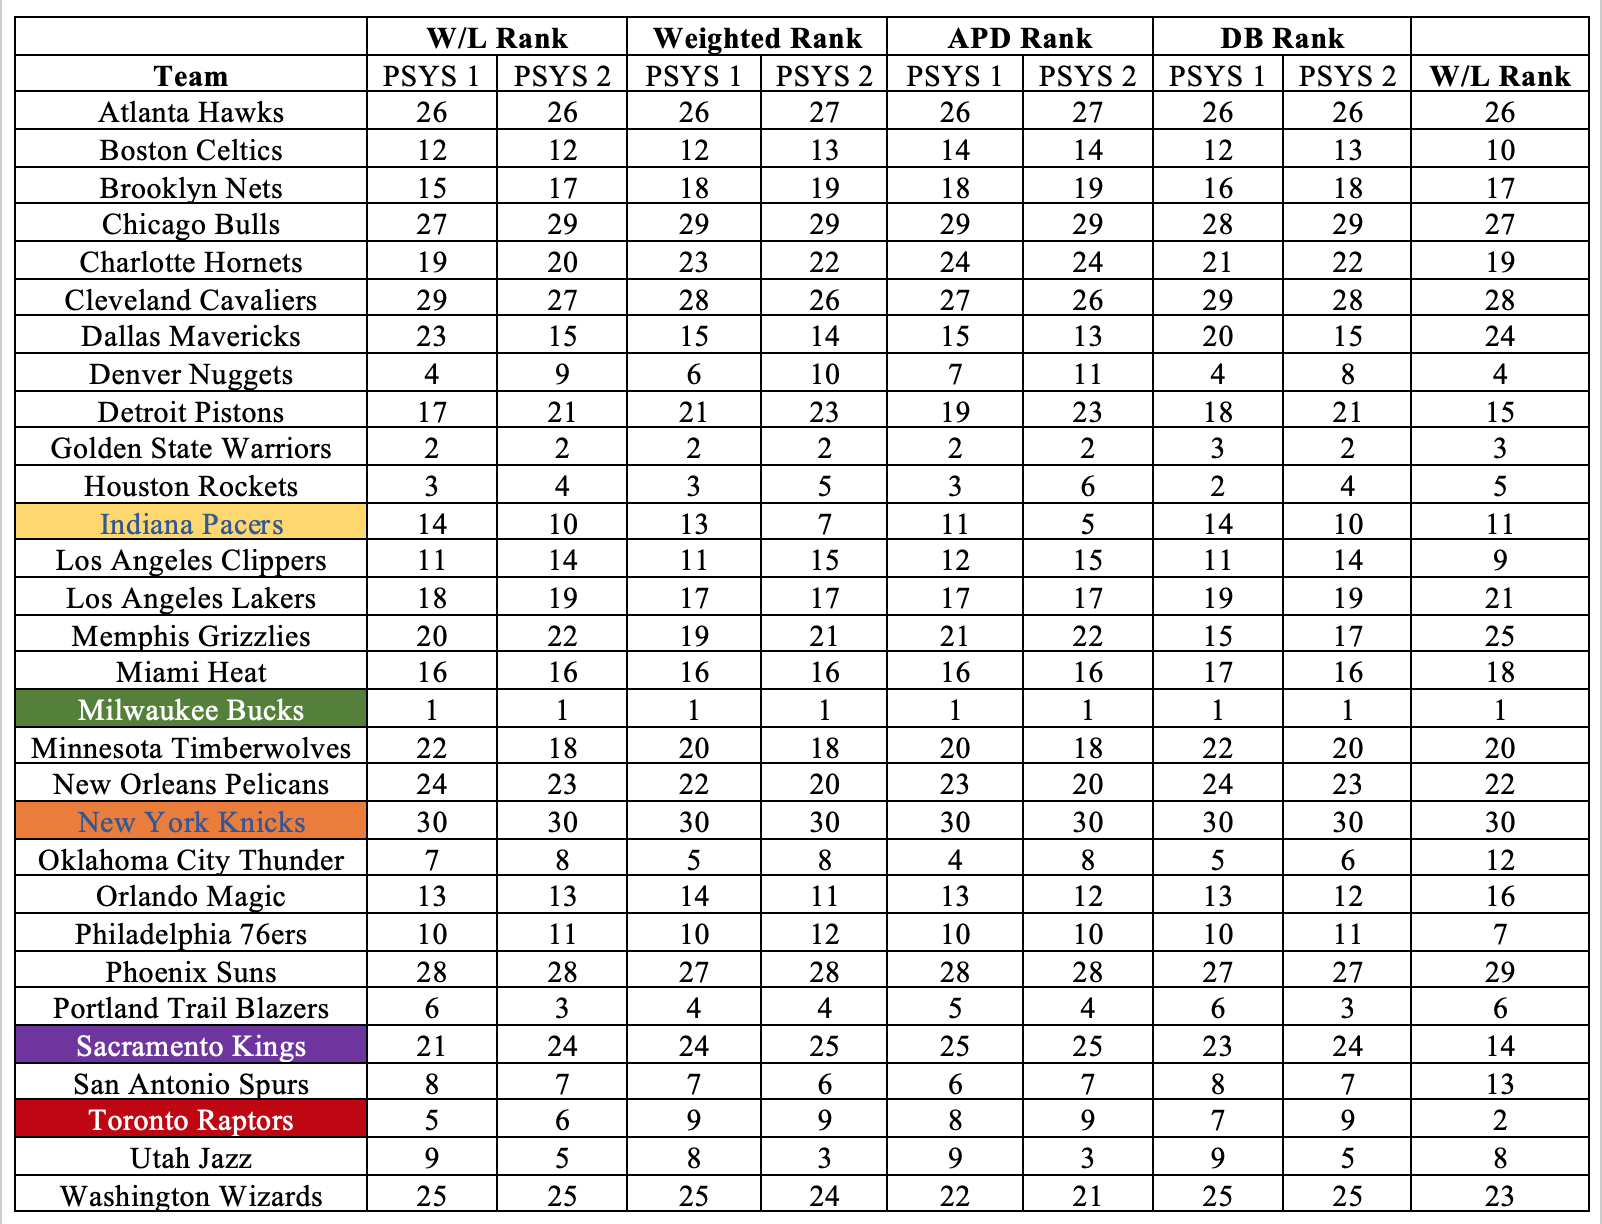
\includegraphics[width=6in]{./images/psys_appendix.png}
  \caption[Ranking of teams after PSYS post-processing]{Ranking of teams after PSYS post-processing}
\end{figure}
\end{document}